% Options for packages loaded elsewhere
\PassOptionsToPackage{unicode}{hyperref}
\PassOptionsToPackage{hyphens}{url}
%
\documentclass[
]{article}
\usepackage{amsmath,amssymb}
\usepackage{iftex}
\ifPDFTeX
  \usepackage[T1]{fontenc}
  \usepackage[utf8]{inputenc}
  \usepackage{textcomp} % provide euro and other symbols
\else % if luatex or xetex
  \usepackage{unicode-math} % this also loads fontspec
  \defaultfontfeatures{Scale=MatchLowercase}
  \defaultfontfeatures[\rmfamily]{Ligatures=TeX,Scale=1}
\fi
\usepackage{lmodern}
\ifPDFTeX\else
  % xetex/luatex font selection
\fi
% Use upquote if available, for straight quotes in verbatim environments
\IfFileExists{upquote.sty}{\usepackage{upquote}}{}
\IfFileExists{microtype.sty}{% use microtype if available
  \usepackage[]{microtype}
  \UseMicrotypeSet[protrusion]{basicmath} % disable protrusion for tt fonts
}{}
\makeatletter
\@ifundefined{KOMAClassName}{% if non-KOMA class
  \IfFileExists{parskip.sty}{%
    \usepackage{parskip}
  }{% else
    \setlength{\parindent}{0pt}
    \setlength{\parskip}{6pt plus 2pt minus 1pt}}
}{% if KOMA class
  \KOMAoptions{parskip=half}}
\makeatother
\usepackage{xcolor}
\usepackage[margin=1in]{geometry}
\usepackage{color}
\usepackage{fancyvrb}
\newcommand{\VerbBar}{|}
\newcommand{\VERB}{\Verb[commandchars=\\\{\}]}
\DefineVerbatimEnvironment{Highlighting}{Verbatim}{commandchars=\\\{\}}
% Add ',fontsize=\small' for more characters per line
\usepackage{framed}
\definecolor{shadecolor}{RGB}{248,248,248}
\newenvironment{Shaded}{\begin{snugshade}}{\end{snugshade}}
\newcommand{\AlertTok}[1]{\textcolor[rgb]{0.94,0.16,0.16}{#1}}
\newcommand{\AnnotationTok}[1]{\textcolor[rgb]{0.56,0.35,0.01}{\textbf{\textit{#1}}}}
\newcommand{\AttributeTok}[1]{\textcolor[rgb]{0.13,0.29,0.53}{#1}}
\newcommand{\BaseNTok}[1]{\textcolor[rgb]{0.00,0.00,0.81}{#1}}
\newcommand{\BuiltInTok}[1]{#1}
\newcommand{\CharTok}[1]{\textcolor[rgb]{0.31,0.60,0.02}{#1}}
\newcommand{\CommentTok}[1]{\textcolor[rgb]{0.56,0.35,0.01}{\textit{#1}}}
\newcommand{\CommentVarTok}[1]{\textcolor[rgb]{0.56,0.35,0.01}{\textbf{\textit{#1}}}}
\newcommand{\ConstantTok}[1]{\textcolor[rgb]{0.56,0.35,0.01}{#1}}
\newcommand{\ControlFlowTok}[1]{\textcolor[rgb]{0.13,0.29,0.53}{\textbf{#1}}}
\newcommand{\DataTypeTok}[1]{\textcolor[rgb]{0.13,0.29,0.53}{#1}}
\newcommand{\DecValTok}[1]{\textcolor[rgb]{0.00,0.00,0.81}{#1}}
\newcommand{\DocumentationTok}[1]{\textcolor[rgb]{0.56,0.35,0.01}{\textbf{\textit{#1}}}}
\newcommand{\ErrorTok}[1]{\textcolor[rgb]{0.64,0.00,0.00}{\textbf{#1}}}
\newcommand{\ExtensionTok}[1]{#1}
\newcommand{\FloatTok}[1]{\textcolor[rgb]{0.00,0.00,0.81}{#1}}
\newcommand{\FunctionTok}[1]{\textcolor[rgb]{0.13,0.29,0.53}{\textbf{#1}}}
\newcommand{\ImportTok}[1]{#1}
\newcommand{\InformationTok}[1]{\textcolor[rgb]{0.56,0.35,0.01}{\textbf{\textit{#1}}}}
\newcommand{\KeywordTok}[1]{\textcolor[rgb]{0.13,0.29,0.53}{\textbf{#1}}}
\newcommand{\NormalTok}[1]{#1}
\newcommand{\OperatorTok}[1]{\textcolor[rgb]{0.81,0.36,0.00}{\textbf{#1}}}
\newcommand{\OtherTok}[1]{\textcolor[rgb]{0.56,0.35,0.01}{#1}}
\newcommand{\PreprocessorTok}[1]{\textcolor[rgb]{0.56,0.35,0.01}{\textit{#1}}}
\newcommand{\RegionMarkerTok}[1]{#1}
\newcommand{\SpecialCharTok}[1]{\textcolor[rgb]{0.81,0.36,0.00}{\textbf{#1}}}
\newcommand{\SpecialStringTok}[1]{\textcolor[rgb]{0.31,0.60,0.02}{#1}}
\newcommand{\StringTok}[1]{\textcolor[rgb]{0.31,0.60,0.02}{#1}}
\newcommand{\VariableTok}[1]{\textcolor[rgb]{0.00,0.00,0.00}{#1}}
\newcommand{\VerbatimStringTok}[1]{\textcolor[rgb]{0.31,0.60,0.02}{#1}}
\newcommand{\WarningTok}[1]{\textcolor[rgb]{0.56,0.35,0.01}{\textbf{\textit{#1}}}}
\usepackage{longtable,booktabs,array}
\usepackage{calc} % for calculating minipage widths
% Correct order of tables after \paragraph or \subparagraph
\usepackage{etoolbox}
\makeatletter
\patchcmd\longtable{\par}{\if@noskipsec\mbox{}\fi\par}{}{}
\makeatother
% Allow footnotes in longtable head/foot
\IfFileExists{footnotehyper.sty}{\usepackage{footnotehyper}}{\usepackage{footnote}}
\makesavenoteenv{longtable}
\usepackage{graphicx}
\makeatletter
\newsavebox\pandoc@box
\newcommand*\pandocbounded[1]{% scales image to fit in text height/width
  \sbox\pandoc@box{#1}%
  \Gscale@div\@tempa{\textheight}{\dimexpr\ht\pandoc@box+\dp\pandoc@box\relax}%
  \Gscale@div\@tempb{\linewidth}{\wd\pandoc@box}%
  \ifdim\@tempb\p@<\@tempa\p@\let\@tempa\@tempb\fi% select the smaller of both
  \ifdim\@tempa\p@<\p@\scalebox{\@tempa}{\usebox\pandoc@box}%
  \else\usebox{\pandoc@box}%
  \fi%
}
% Set default figure placement to htbp
\def\fps@figure{htbp}
\makeatother
\setlength{\emergencystretch}{3em} % prevent overfull lines
\providecommand{\tightlist}{%
  \setlength{\itemsep}{0pt}\setlength{\parskip}{0pt}}
\setcounter{secnumdepth}{-\maxdimen} % remove section numbering
\usepackage{bookmark}
\IfFileExists{xurl.sty}{\usepackage{xurl}}{} % add URL line breaks if available
\urlstyle{same}
\hypersetup{
  hidelinks,
  pdfcreator={LaTeX via pandoc}}

\author{}
\date{\vspace{-2.5em}}

\begin{document}

\section{Introduction}\label{introduction}

\subsection{Principe et définitions}\label{principe-et-duxe9finitions}

Toute modélisation part d'une question de la forme : \textbf{Quel est
l'impact de X sur Y étant donné Z ?}

dans laquelle : - X définit l'ensemble des scénarios à explorer - Y
l'ensemble des indicateurs à observer - Z le contexte de la question

\subsubsection{Concepts fondamentaux}\label{concepts-fondamentaux}

\begin{itemize}
\tightlist
\item
  \textbf{Système} : Système structuré en entités et processus
\end{itemize}

\textbf{Types d'attributs} : - \textbf{parametres} : Valeur fixe durant
la simulation - \textbf{variables\_etat} : Valeur variant au cours du
temps

\textbf{Portée des attributs} : - globaux : partagés par tout le système
- locaux : partagés par entités de même type - individuels : spécifiques
à chaque entité

\subsubsection{Relations
questions-modèle}\label{relations-questions-moduxe8le}

\textbf{Formalisation} :

\begin{verbatim}
X ⊆ A, Z ⊆ A, X ∩ Z = ∅, X ∪ Z = A
\end{verbatim}

\begin{verbatim}
Y est calculé à partir des attributs
\end{verbatim}

\textbf{Implication} : Un choix différent de X et Z permet de répondre à
d'autres questions avec le même modèle

\subsection{Le modèle}\label{le-moduxe8le}

La question retenue pour le modèle est : \textbf{Quel est l'impact des
schémas de gestion et des facteurs exogènes sur la durabilité des
ressources naturelles ?}

\textbf{Domaine} : socio-écosystème agricole \textbf{Échelle} :
territoriale

\subsubsection{Représentations
graphiques}\label{repruxe9sentations-graphiques}

\pandocbounded{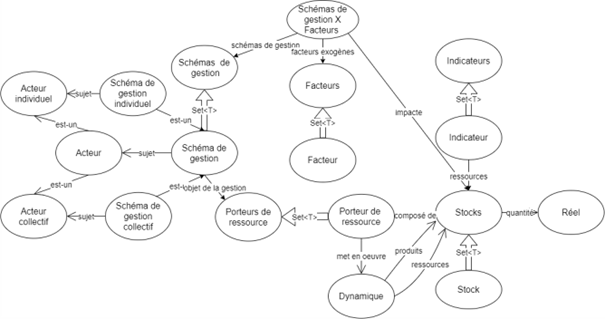
\includegraphics[keepaspectratio]{C:/Users/tingo/source/repos/tingourosanogo/CIM-PIM_Transformation/CIM-PIM_Transformation/project_root/src/input/diagrammes/question.png}}
\textbf{Figure 1} : Question de recherche schématisée

Sur la flèche diagonale, on représente qu'une combinaison (X) de schémas
de gestion et de facteurs impacte les stocks.

\pandocbounded{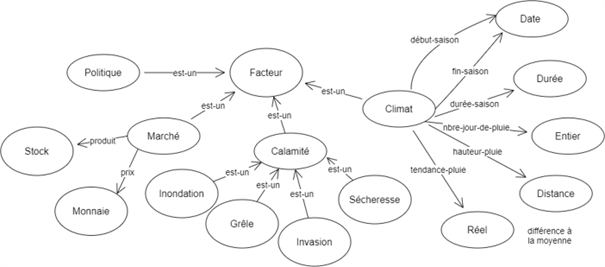
\includegraphics[keepaspectratio]{C:/Users/tingo/source/repos/tingourosanogo/CIM-PIM_Transformation/CIM-PIM_Transformation/project_root/src/input/diagrammes/facteurs.png}}
\textbf{Figure 2} : Facteurs exogènes

Les facteurs exogènes sont un ensemble de facteurs influençant le
système sans être contrôlés par les acteurs.

\subsubsection{Composants principaux}\label{composants-principaux}

\paragraph{Porteurs\_Ressources}\label{porteurs_ressources}

\textbf{Description} : Composés de divers stocks et mettent en œuvre des
dynamiques \textbf{Rôle} : Utilisent des stocks comme ressources et
produisent des stocks

\paragraph{Schemas\_Gestion}\label{schemas_gestion}

\textbf{Description} : Ensembles de schémas de gestion mis en œuvre par
des acteurs \textbf{Types} : - individuels : par exploitation -
collectifs : par village

\paragraph{Stocks}\label{stocks}

\textbf{Description} : Quantités de ressources pour différents usages
\textbf{Usages} : - humains - animaux - plantes - processus biophysiques

\subsubsection{Acteurs du système}\label{acteurs-du-systuxe8me}

\begin{itemize}
\tightlist
\item
  \textbf{Individuels} : exploitations agricoles
\item
  \textbf{Collectifs} : villages, coopératives
\end{itemize}

\subsection{Contextualisation}\label{contextualisation}

\textbf{Domaine d'application} : agroécologie, gestion des ressources
naturelles

\textbf{Pertinence scientifique} : Modélisation des interactions
complexes entre pratiques de gestion et dynamiques des ressources dans
un contexte de changement global

\textbf{Public cible} : - décideurs politiques - chercheurs en
socio-écosystèmes - acteurs territoriaux

\section{Structure et dynamique}\label{structure-et-dynamique}

\subsection{Entité : Actor}\label{entituxe9-actor}

\subsubsection{Documentation}\label{documentation}

\emph{Description à compléter}

\subsubsection{Attributs}\label{attributs}

\textbf{Attributs partagés (fixes)}

Les attributs dont la valeur est la même pour toutes les instances et
fixe dans la simulation :

\begin{longtable}[]{@{}lll@{}}
\toprule\noalign{}
\textbf{Paramètre} & \textbf{Commentaire} & \textbf{Unité} \\
\midrule\noalign{}
\endhead
\bottomrule\noalign{}
\endlastfoot
\ldots{} & \ldots{} & \ldots{} \\
\end{longtable}

\textbf{Variables partagées}

Les variables dont la valeur est la même pour toutes les instances et
évolue au cours de la simulation :

\begin{longtable}[]{@{}lll@{}}
\toprule\noalign{}
\textbf{Paramètre} & \textbf{Commentaire} & \textbf{Unité} \\
\midrule\noalign{}
\endhead
\bottomrule\noalign{}
\endlastfoot
\ldots{} & \ldots{} & \ldots{} \\
\end{longtable}

\textbf{Attributs individuels}

Les attributs dont la valeur est différente pour chaque instance et
évolue au cours de la simulation :

\begin{longtable}[]{@{}lll@{}}
\toprule\noalign{}
\textbf{Paramètre} & \textbf{Commentaire} & \textbf{Unité} \\
\midrule\noalign{}
\endhead
\bottomrule\noalign{}
\endlastfoot
\ldots{} & \ldots{} & \ldots{} \\
\end{longtable}

\textbf{Variables individuelles (fixes)}

Les attributs dont la valeur est différente pour chaque instance et fixe
dans la simulation :

\begin{longtable}[]{@{}lll@{}}
\toprule\noalign{}
\textbf{Paramètre} & \textbf{Commentaire} & \textbf{Unité} \\
\midrule\noalign{}
\endhead
\bottomrule\noalign{}
\endlastfoot
\texttt{id} & \ldots{} & string \\
\texttt{type} & \ldots{} & string \\
\end{longtable}

\subsubsection{Questions ouvertes}\label{questions-ouvertes}

\emph{Liste des points à discuter.}

\emph{Section vide : à compléter manuellement}

\subsubsection{Dynamiques}\label{dynamiques}

\emph{Section vide : à compléter manuellement}

\subsection{Entité : IndividualActor}\label{entituxe9-individualactor}

\subsubsection{Documentation}\label{documentation-1}

\emph{Description à compléter}

\subsubsection{Attributs}\label{attributs-1}

\textbf{Attributs partagés (fixes)}

Les attributs dont la valeur est la même pour toutes les instances et
fixe dans la simulation :

\begin{longtable}[]{@{}lll@{}}
\toprule\noalign{}
\textbf{Paramètre} & \textbf{Commentaire} & \textbf{Unité} \\
\midrule\noalign{}
\endhead
\bottomrule\noalign{}
\endlastfoot
\ldots{} & \ldots{} & \ldots{} \\
\end{longtable}

\textbf{Variables partagées}

Les variables dont la valeur est la même pour toutes les instances et
évolue au cours de la simulation :

\begin{longtable}[]{@{}lll@{}}
\toprule\noalign{}
\textbf{Paramètre} & \textbf{Commentaire} & \textbf{Unité} \\
\midrule\noalign{}
\endhead
\bottomrule\noalign{}
\endlastfoot
\ldots{} & \ldots{} & \ldots{} \\
\end{longtable}

\textbf{Attributs individuels}

Les attributs dont la valeur est différente pour chaque instance et
évolue au cours de la simulation :

\begin{longtable}[]{@{}lll@{}}
\toprule\noalign{}
\textbf{Paramètre} & \textbf{Commentaire} & \textbf{Unité} \\
\midrule\noalign{}
\endhead
\bottomrule\noalign{}
\endlastfoot
\ldots{} & \ldots{} & \ldots{} \\
\end{longtable}

\textbf{Variables individuelles (fixes)}

Les attributs dont la valeur est différente pour chaque instance et fixe
dans la simulation :

\begin{longtable}[]{@{}lll@{}}
\toprule\noalign{}
\textbf{Paramètre} & \textbf{Commentaire} & \textbf{Unité} \\
\midrule\noalign{}
\endhead
\bottomrule\noalign{}
\endlastfoot
\ldots{} & \ldots{} & \ldots{} \\
\end{longtable}

\subsubsection{Questions ouvertes}\label{questions-ouvertes-1}

\emph{Liste des points à discuter.}

\emph{Section vide : à compléter manuellement}

\subsubsection{Dynamiques}\label{dynamiques-1}

\paragraph{\texorpdfstring{\emph{Processus:
manageResource}}{Processus: manageResource}}\label{processus-manageresource}

\subparagraph{Documentation :}\label{documentation-2}

\emph{Description à compléter}

\subparagraph{Attributs}\label{attributs-2}

Le processus dépend des variables suivantes :

\begin{longtable}[]{@{}llll@{}}
\toprule\noalign{}
\textbf{Variables d'état} & \textbf{Entité} & \textbf{Définition} &
\textbf{Unité} \\
\midrule\noalign{}
\endhead
\bottomrule\noalign{}
\endlastfoot
\ldots{} & \ldots{} & \ldots{} & \ldots{} \\
\end{longtable}

Le processus agit sur les variables suivantes :

\begin{longtable}[]{@{}llll@{}}
\toprule\noalign{}
\textbf{Variables d'état} & \textbf{Entité} & \textbf{Définition} &
\textbf{Unité} \\
\midrule\noalign{}
\endhead
\bottomrule\noalign{}
\endlastfoot
\ldots{} & \ldots{} & \ldots{} & \ldots{} \\
\end{longtable}

et dépend des paramètres suivants :

\begin{longtable}[]{@{}llll@{}}
\toprule\noalign{}
\textbf{Paramètres} & \textbf{Entité} & \textbf{Définition} &
\textbf{Unité} \\
\midrule\noalign{}
\endhead
\bottomrule\noalign{}
\endlastfoot
\ldots{} & \ldots{} & \ldots{} & \ldots{} \\
\end{longtable}

\subparagraph{Comportement}\label{comportement}

\emph{Description détaillée du processus avec, éventuellement des
sous-processus, des équations, des diagrammes d'état ou d'activité
(UML), etc.}

Équation : \emph{A compléter}

Diagramme : \emph{A compléter}

\subparagraph{Code}\label{code}

\emph{Le code ou pseudo-code s'il existe pour ceux qui peuvent le
comprendre.}

\emph{A compléter}

\subsection{Entité : Resource}\label{entituxe9-resource}

\subsubsection{Documentation}\label{documentation-3}

\emph{Description à compléter}

\subsubsection{Attributs}\label{attributs-3}

\textbf{Attributs partagés (fixes)}

Les attributs dont la valeur est la même pour toutes les instances et
fixe dans la simulation :

\begin{longtable}[]{@{}lll@{}}
\toprule\noalign{}
\textbf{Paramètre} & \textbf{Commentaire} & \textbf{Unité} \\
\midrule\noalign{}
\endhead
\bottomrule\noalign{}
\endlastfoot
\ldots{} & \ldots{} & \ldots{} \\
\end{longtable}

\textbf{Variables partagées}

Les variables dont la valeur est la même pour toutes les instances et
évolue au cours de la simulation :

\begin{longtable}[]{@{}lll@{}}
\toprule\noalign{}
\textbf{Paramètre} & \textbf{Commentaire} & \textbf{Unité} \\
\midrule\noalign{}
\endhead
\bottomrule\noalign{}
\endlastfoot
\ldots{} & \ldots{} & \ldots{} \\
\end{longtable}

\textbf{Attributs individuels}

Les attributs dont la valeur est différente pour chaque instance et
évolue au cours de la simulation :

\begin{longtable}[]{@{}lll@{}}
\toprule\noalign{}
\textbf{Paramètre} & \textbf{Commentaire} & \textbf{Unité} \\
\midrule\noalign{}
\endhead
\bottomrule\noalign{}
\endlastfoot
\ldots{} & \ldots{} & \ldots{} \\
\end{longtable}

\textbf{Variables individuelles (fixes)}

Les attributs dont la valeur est différente pour chaque instance et fixe
dans la simulation :

\begin{longtable}[]{@{}lll@{}}
\toprule\noalign{}
\textbf{Paramètre} & \textbf{Commentaire} & \textbf{Unité} \\
\midrule\noalign{}
\endhead
\bottomrule\noalign{}
\endlastfoot
\texttt{id} & \ldots{} & string \\
\texttt{quantity} & \ldots{} & float \\
\end{longtable}

\subsubsection{Questions ouvertes}\label{questions-ouvertes-2}

\emph{Liste des points à discuter.}

\emph{Section vide : à compléter manuellement}

\subsubsection{Dynamiques}\label{dynamiques-2}

\emph{Section vide : à compléter manuellement}

\subsection{Entité : FarmingActivity}\label{entituxe9-farmingactivity}

\subsubsection{Documentation}\label{documentation-4}

\emph{Description à compléter}

\subsubsection{Attributs}\label{attributs-4}

\textbf{Attributs partagés (fixes)}

Les attributs dont la valeur est la même pour toutes les instances et
fixe dans la simulation :

\begin{longtable}[]{@{}lll@{}}
\toprule\noalign{}
\textbf{Paramètre} & \textbf{Commentaire} & \textbf{Unité} \\
\midrule\noalign{}
\endhead
\bottomrule\noalign{}
\endlastfoot
\ldots{} & \ldots{} & \ldots{} \\
\end{longtable}

\textbf{Variables partagées}

Les variables dont la valeur est la même pour toutes les instances et
évolue au cours de la simulation :

\begin{longtable}[]{@{}lll@{}}
\toprule\noalign{}
\textbf{Paramètre} & \textbf{Commentaire} & \textbf{Unité} \\
\midrule\noalign{}
\endhead
\bottomrule\noalign{}
\endlastfoot
\ldots{} & \ldots{} & \ldots{} \\
\end{longtable}

\textbf{Attributs individuels}

Les attributs dont la valeur est différente pour chaque instance et
évolue au cours de la simulation :

\begin{longtable}[]{@{}lll@{}}
\toprule\noalign{}
\textbf{Paramètre} & \textbf{Commentaire} & \textbf{Unité} \\
\midrule\noalign{}
\endhead
\bottomrule\noalign{}
\endlastfoot
\ldots{} & \ldots{} & \ldots{} \\
\end{longtable}

\textbf{Variables individuelles (fixes)}

Les attributs dont la valeur est différente pour chaque instance et fixe
dans la simulation :

\begin{longtable}[]{@{}lll@{}}
\toprule\noalign{}
\textbf{Paramètre} & \textbf{Commentaire} & \textbf{Unité} \\
\midrule\noalign{}
\endhead
\bottomrule\noalign{}
\endlastfoot
\texttt{startDate} & \ldots{} & date \\
\texttt{endDate} & \ldots{} & date \\
\end{longtable}

\subsubsection{Questions ouvertes}\label{questions-ouvertes-3}

\emph{Liste des points à discuter.}

\emph{Section vide : à compléter manuellement}

\subsubsection{Dynamiques}\label{dynamiques-3}

\emph{Section vide : à compléter manuellement}

\subsection{Entité : Livestock}\label{entituxe9-livestock}

\subsubsection{Documentation}\label{documentation-5}

\emph{Description à compléter}

\subsubsection{Attributs}\label{attributs-5}

\textbf{Attributs partagés (fixes)}

Les attributs dont la valeur est la même pour toutes les instances et
fixe dans la simulation :

\begin{longtable}[]{@{}lll@{}}
\toprule\noalign{}
\textbf{Paramètre} & \textbf{Commentaire} & \textbf{Unité} \\
\midrule\noalign{}
\endhead
\bottomrule\noalign{}
\endlastfoot
\ldots{} & \ldots{} & \ldots{} \\
\end{longtable}

\textbf{Variables partagées}

Les variables dont la valeur est la même pour toutes les instances et
évolue au cours de la simulation :

\begin{longtable}[]{@{}lll@{}}
\toprule\noalign{}
\textbf{Paramètre} & \textbf{Commentaire} & \textbf{Unité} \\
\midrule\noalign{}
\endhead
\bottomrule\noalign{}
\endlastfoot
\ldots{} & \ldots{} & \ldots{} \\
\end{longtable}

\textbf{Attributs individuels}

Les attributs dont la valeur est différente pour chaque instance et
évolue au cours de la simulation :

\begin{longtable}[]{@{}lll@{}}
\toprule\noalign{}
\textbf{Paramètre} & \textbf{Commentaire} & \textbf{Unité} \\
\midrule\noalign{}
\endhead
\bottomrule\noalign{}
\endlastfoot
\ldots{} & \ldots{} & \ldots{} \\
\end{longtable}

\textbf{Variables individuelles (fixes)}

Les attributs dont la valeur est différente pour chaque instance et fixe
dans la simulation :

\begin{longtable}[]{@{}lll@{}}
\toprule\noalign{}
\textbf{Paramètre} & \textbf{Commentaire} & \textbf{Unité} \\
\midrule\noalign{}
\endhead
\bottomrule\noalign{}
\endlastfoot
\texttt{herdSize} & \ldots{} & integer \\
\end{longtable}

\subsubsection{Questions ouvertes}\label{questions-ouvertes-4}

\emph{Liste des points à discuter.}

\emph{Section vide : à compléter manuellement}

\subsubsection{Dynamiques}\label{dynamiques-4}

\paragraph{\texorpdfstring{\emph{Processus:
produceMeat}}{Processus: produceMeat}}\label{processus-producemeat}

\subparagraph{Documentation :}\label{documentation-6}

\emph{Description à compléter}

\subparagraph{Attributs}\label{attributs-6}

Le processus dépend des variables suivantes :

\begin{longtable}[]{@{}llll@{}}
\toprule\noalign{}
\textbf{Variables d'état} & \textbf{Entité} & \textbf{Définition} &
\textbf{Unité} \\
\midrule\noalign{}
\endhead
\bottomrule\noalign{}
\endlastfoot
\ldots{} & \ldots{} & \ldots{} & \ldots{} \\
\end{longtable}

Le processus agit sur les variables suivantes :

\begin{longtable}[]{@{}llll@{}}
\toprule\noalign{}
\textbf{Variables d'état} & \textbf{Entité} & \textbf{Définition} &
\textbf{Unité} \\
\midrule\noalign{}
\endhead
\bottomrule\noalign{}
\endlastfoot
\ldots{} & \ldots{} & \ldots{} & \ldots{} \\
\end{longtable}

et dépend des paramètres suivants :

\begin{longtable}[]{@{}llll@{}}
\toprule\noalign{}
\textbf{Paramètres} & \textbf{Entité} & \textbf{Définition} &
\textbf{Unité} \\
\midrule\noalign{}
\endhead
\bottomrule\noalign{}
\endlastfoot
\ldots{} & \ldots{} & \ldots{} & \ldots{} \\
\end{longtable}

\subparagraph{Comportement}\label{comportement-1}

\emph{Description détaillée du processus avec, éventuellement des
sous-processus, des équations, des diagrammes d'état ou d'activité
(UML), etc.}

Équation : \emph{A compléter}

Diagramme : \emph{A compléter}

\subparagraph{Code}\label{code-1}

\emph{Le code ou pseudo-code s'il existe pour ceux qui peuvent le
comprendre.}

\emph{A compléter}

\paragraph{\texorpdfstring{\emph{Processus:
produceMilk}}{Processus: produceMilk}}\label{processus-producemilk}

\subparagraph{Documentation :}\label{documentation-7}

\emph{Description à compléter}

\subparagraph{Attributs}\label{attributs-7}

Le processus dépend des variables suivantes :

\begin{longtable}[]{@{}llll@{}}
\toprule\noalign{}
\textbf{Variables d'état} & \textbf{Entité} & \textbf{Définition} &
\textbf{Unité} \\
\midrule\noalign{}
\endhead
\bottomrule\noalign{}
\endlastfoot
\ldots{} & \ldots{} & \ldots{} & \ldots{} \\
\end{longtable}

Le processus agit sur les variables suivantes :

\begin{longtable}[]{@{}llll@{}}
\toprule\noalign{}
\textbf{Variables d'état} & \textbf{Entité} & \textbf{Définition} &
\textbf{Unité} \\
\midrule\noalign{}
\endhead
\bottomrule\noalign{}
\endlastfoot
\ldots{} & \ldots{} & \ldots{} & \ldots{} \\
\end{longtable}

et dépend des paramètres suivants :

\begin{longtable}[]{@{}llll@{}}
\toprule\noalign{}
\textbf{Paramètres} & \textbf{Entité} & \textbf{Définition} &
\textbf{Unité} \\
\midrule\noalign{}
\endhead
\bottomrule\noalign{}
\endlastfoot
\ldots{} & \ldots{} & \ldots{} & \ldots{} \\
\end{longtable}

\subparagraph{Comportement}\label{comportement-2}

\emph{Description détaillée du processus avec, éventuellement des
sous-processus, des équations, des diagrammes d'état ou d'activité
(UML), etc.}

Équation : \emph{A compléter}

Diagramme : \emph{A compléter}

\subparagraph{Code}\label{code-2}

\emph{Le code ou pseudo-code s'il existe pour ceux qui peuvent le
comprendre.}

\emph{A compléter}

\subsection{Entité : Plant}\label{entituxe9-plant}

\subsubsection{Documentation}\label{documentation-8}

\emph{Description à compléter}

\subsubsection{Attributs}\label{attributs-8}

\textbf{Attributs partagés (fixes)}

Les attributs dont la valeur est la même pour toutes les instances et
fixe dans la simulation :

\begin{longtable}[]{@{}lll@{}}
\toprule\noalign{}
\textbf{Paramètre} & \textbf{Commentaire} & \textbf{Unité} \\
\midrule\noalign{}
\endhead
\bottomrule\noalign{}
\endlastfoot
\ldots{} & \ldots{} & \ldots{} \\
\end{longtable}

\textbf{Variables partagées}

Les variables dont la valeur est la même pour toutes les instances et
évolue au cours de la simulation :

\begin{longtable}[]{@{}lll@{}}
\toprule\noalign{}
\textbf{Paramètre} & \textbf{Commentaire} & \textbf{Unité} \\
\midrule\noalign{}
\endhead
\bottomrule\noalign{}
\endlastfoot
\ldots{} & \ldots{} & \ldots{} \\
\end{longtable}

\textbf{Attributs individuels}

Les attributs dont la valeur est différente pour chaque instance et
évolue au cours de la simulation :

\begin{longtable}[]{@{}lll@{}}
\toprule\noalign{}
\textbf{Paramètre} & \textbf{Commentaire} & \textbf{Unité} \\
\midrule\noalign{}
\endhead
\bottomrule\noalign{}
\endlastfoot
\ldots{} & \ldots{} & \ldots{} \\
\end{longtable}

\textbf{Variables individuelles (fixes)}

Les attributs dont la valeur est différente pour chaque instance et fixe
dans la simulation :

\begin{longtable}[]{@{}lll@{}}
\toprule\noalign{}
\textbf{Paramètre} & \textbf{Commentaire} & \textbf{Unité} \\
\midrule\noalign{}
\endhead
\bottomrule\noalign{}
\endlastfoot
\texttt{species} & \ldots{} & string \\
\texttt{biomass} & \ldots{} & float \\
\end{longtable}

\subsubsection{Questions ouvertes}\label{questions-ouvertes-5}

\emph{Liste des points à discuter.}

\emph{Section vide : à compléter manuellement}

\subsubsection{Dynamiques}\label{dynamiques-5}

\paragraph{\texorpdfstring{\emph{Processus:
absorbNutrients}}{Processus: absorbNutrients}}\label{processus-absorbnutrients}

\subparagraph{Documentation :}\label{documentation-9}

\emph{Description à compléter}

\subparagraph{Attributs}\label{attributs-9}

Le processus dépend des variables suivantes :

\begin{longtable}[]{@{}llll@{}}
\toprule\noalign{}
\textbf{Variables d'état} & \textbf{Entité} & \textbf{Définition} &
\textbf{Unité} \\
\midrule\noalign{}
\endhead
\bottomrule\noalign{}
\endlastfoot
\ldots{} & \ldots{} & \ldots{} & \ldots{} \\
\end{longtable}

Le processus agit sur les variables suivantes :

\begin{longtable}[]{@{}llll@{}}
\toprule\noalign{}
\textbf{Variables d'état} & \textbf{Entité} & \textbf{Définition} &
\textbf{Unité} \\
\midrule\noalign{}
\endhead
\bottomrule\noalign{}
\endlastfoot
\ldots{} & \ldots{} & \ldots{} & \ldots{} \\
\end{longtable}

et dépend des paramètres suivants :

\begin{longtable}[]{@{}llll@{}}
\toprule\noalign{}
\textbf{Paramètres} & \textbf{Entité} & \textbf{Définition} &
\textbf{Unité} \\
\midrule\noalign{}
\endhead
\bottomrule\noalign{}
\endlastfoot
\ldots{} & \ldots{} & \ldots{} & \ldots{} \\
\end{longtable}

\subparagraph{Comportement}\label{comportement-3}

\emph{Description détaillée du processus avec, éventuellement des
sous-processus, des équations, des diagrammes d'état ou d'activité
(UML), etc.}

Équation : \emph{A compléter}

Diagramme : \emph{A compléter}

\subparagraph{Code}\label{code-3}

\emph{Le code ou pseudo-code s'il existe pour ceux qui peuvent le
comprendre.}

\emph{A compléter}

\subsection{Entité : Product}\label{entituxe9-product}

\subsubsection{Documentation}\label{documentation-10}

\emph{Description à compléter}

\subsubsection{Attributs}\label{attributs-10}

\textbf{Attributs partagés (fixes)}

Les attributs dont la valeur est la même pour toutes les instances et
fixe dans la simulation :

\begin{longtable}[]{@{}lll@{}}
\toprule\noalign{}
\textbf{Paramètre} & \textbf{Commentaire} & \textbf{Unité} \\
\midrule\noalign{}
\endhead
\bottomrule\noalign{}
\endlastfoot
\ldots{} & \ldots{} & \ldots{} \\
\end{longtable}

\textbf{Variables partagées}

Les variables dont la valeur est la même pour toutes les instances et
évolue au cours de la simulation :

\begin{longtable}[]{@{}lll@{}}
\toprule\noalign{}
\textbf{Paramètre} & \textbf{Commentaire} & \textbf{Unité} \\
\midrule\noalign{}
\endhead
\bottomrule\noalign{}
\endlastfoot
\ldots{} & \ldots{} & \ldots{} \\
\end{longtable}

\textbf{Attributs individuels}

Les attributs dont la valeur est différente pour chaque instance et
évolue au cours de la simulation :

\begin{longtable}[]{@{}lll@{}}
\toprule\noalign{}
\textbf{Paramètre} & \textbf{Commentaire} & \textbf{Unité} \\
\midrule\noalign{}
\endhead
\bottomrule\noalign{}
\endlastfoot
\ldots{} & \ldots{} & \ldots{} \\
\end{longtable}

\textbf{Variables individuelles (fixes)}

Les attributs dont la valeur est différente pour chaque instance et fixe
dans la simulation :

\begin{longtable}[]{@{}lll@{}}
\toprule\noalign{}
\textbf{Paramètre} & \textbf{Commentaire} & \textbf{Unité} \\
\midrule\noalign{}
\endhead
\bottomrule\noalign{}
\endlastfoot
\texttt{quality} & \ldots{} & float \\
\end{longtable}

\subsubsection{Questions ouvertes}\label{questions-ouvertes-6}

\emph{Liste des points à discuter.}

\emph{Section vide : à compléter manuellement}

\subsubsection{Dynamiques}\label{dynamiques-6}

\emph{Section vide : à compléter manuellement}

\subsection{Entité : Meat}\label{entituxe9-meat}

\subsubsection{Documentation}\label{documentation-11}

\emph{Description à compléter}

\subsubsection{Attributs}\label{attributs-11}

\textbf{Attributs partagés (fixes)}

Les attributs dont la valeur est la même pour toutes les instances et
fixe dans la simulation :

\begin{longtable}[]{@{}lll@{}}
\toprule\noalign{}
\textbf{Paramètre} & \textbf{Commentaire} & \textbf{Unité} \\
\midrule\noalign{}
\endhead
\bottomrule\noalign{}
\endlastfoot
\ldots{} & \ldots{} & \ldots{} \\
\end{longtable}

\textbf{Variables partagées}

Les variables dont la valeur est la même pour toutes les instances et
évolue au cours de la simulation :

\begin{longtable}[]{@{}lll@{}}
\toprule\noalign{}
\textbf{Paramètre} & \textbf{Commentaire} & \textbf{Unité} \\
\midrule\noalign{}
\endhead
\bottomrule\noalign{}
\endlastfoot
\ldots{} & \ldots{} & \ldots{} \\
\end{longtable}

\textbf{Attributs individuels}

Les attributs dont la valeur est différente pour chaque instance et
évolue au cours de la simulation :

\begin{longtable}[]{@{}lll@{}}
\toprule\noalign{}
\textbf{Paramètre} & \textbf{Commentaire} & \textbf{Unité} \\
\midrule\noalign{}
\endhead
\bottomrule\noalign{}
\endlastfoot
\ldots{} & \ldots{} & \ldots{} \\
\end{longtable}

\textbf{Variables individuelles (fixes)}

Les attributs dont la valeur est différente pour chaque instance et fixe
dans la simulation :

\begin{longtable}[]{@{}lll@{}}
\toprule\noalign{}
\textbf{Paramètre} & \textbf{Commentaire} & \textbf{Unité} \\
\midrule\noalign{}
\endhead
\bottomrule\noalign{}
\endlastfoot
\texttt{cutType} & \ldots{} & string \\
\end{longtable}

\subsubsection{Questions ouvertes}\label{questions-ouvertes-7}

\emph{Liste des points à discuter.}

\emph{Section vide : à compléter manuellement}

\subsubsection{Dynamiques}\label{dynamiques-7}

\emph{Section vide : à compléter manuellement}

\subsection{Entité : Milk}\label{entituxe9-milk}

\subsubsection{Documentation}\label{documentation-12}

\emph{Description à compléter}

\subsubsection{Attributs}\label{attributs-12}

\textbf{Attributs partagés (fixes)}

Les attributs dont la valeur est la même pour toutes les instances et
fixe dans la simulation :

\begin{longtable}[]{@{}lll@{}}
\toprule\noalign{}
\textbf{Paramètre} & \textbf{Commentaire} & \textbf{Unité} \\
\midrule\noalign{}
\endhead
\bottomrule\noalign{}
\endlastfoot
\ldots{} & \ldots{} & \ldots{} \\
\end{longtable}

\textbf{Variables partagées}

Les variables dont la valeur est la même pour toutes les instances et
évolue au cours de la simulation :

\begin{longtable}[]{@{}lll@{}}
\toprule\noalign{}
\textbf{Paramètre} & \textbf{Commentaire} & \textbf{Unité} \\
\midrule\noalign{}
\endhead
\bottomrule\noalign{}
\endlastfoot
\ldots{} & \ldots{} & \ldots{} \\
\end{longtable}

\textbf{Attributs individuels}

Les attributs dont la valeur est différente pour chaque instance et
évolue au cours de la simulation :

\begin{longtable}[]{@{}lll@{}}
\toprule\noalign{}
\textbf{Paramètre} & \textbf{Commentaire} & \textbf{Unité} \\
\midrule\noalign{}
\endhead
\bottomrule\noalign{}
\endlastfoot
\ldots{} & \ldots{} & \ldots{} \\
\end{longtable}

\textbf{Variables individuelles (fixes)}

Les attributs dont la valeur est différente pour chaque instance et fixe
dans la simulation :

\begin{longtable}[]{@{}lll@{}}
\toprule\noalign{}
\textbf{Paramètre} & \textbf{Commentaire} & \textbf{Unité} \\
\midrule\noalign{}
\endhead
\bottomrule\noalign{}
\endlastfoot
\texttt{fatContent} & \ldots{} & float \\
\end{longtable}

\subsubsection{Questions ouvertes}\label{questions-ouvertes-8}

\emph{Liste des points à discuter.}

\emph{Section vide : à compléter manuellement}

\subsubsection{Dynamiques}\label{dynamiques-8}

\emph{Section vide : à compléter manuellement}

\subsection{Entité : WaterSource}\label{entituxe9-watersource}

\subsubsection{Documentation}\label{documentation-13}

\emph{Description à compléter}

\subsubsection{Attributs}\label{attributs-13}

\textbf{Attributs partagés (fixes)}

Les attributs dont la valeur est la même pour toutes les instances et
fixe dans la simulation :

\begin{longtable}[]{@{}lll@{}}
\toprule\noalign{}
\textbf{Paramètre} & \textbf{Commentaire} & \textbf{Unité} \\
\midrule\noalign{}
\endhead
\bottomrule\noalign{}
\endlastfoot
\ldots{} & \ldots{} & \ldots{} \\
\end{longtable}

\textbf{Variables partagées}

Les variables dont la valeur est la même pour toutes les instances et
évolue au cours de la simulation :

\begin{longtable}[]{@{}lll@{}}
\toprule\noalign{}
\textbf{Paramètre} & \textbf{Commentaire} & \textbf{Unité} \\
\midrule\noalign{}
\endhead
\bottomrule\noalign{}
\endlastfoot
\ldots{} & \ldots{} & \ldots{} \\
\end{longtable}

\textbf{Attributs individuels}

Les attributs dont la valeur est différente pour chaque instance et
évolue au cours de la simulation :

\begin{longtable}[]{@{}lll@{}}
\toprule\noalign{}
\textbf{Paramètre} & \textbf{Commentaire} & \textbf{Unité} \\
\midrule\noalign{}
\endhead
\bottomrule\noalign{}
\endlastfoot
\ldots{} & \ldots{} & \ldots{} \\
\end{longtable}

\textbf{Variables individuelles (fixes)}

Les attributs dont la valeur est différente pour chaque instance et fixe
dans la simulation :

\begin{longtable}[]{@{}lll@{}}
\toprule\noalign{}
\textbf{Paramètre} & \textbf{Commentaire} & \textbf{Unité} \\
\midrule\noalign{}
\endhead
\bottomrule\noalign{}
\endlastfoot
\texttt{capacity} & \ldots{} & float \\
\end{longtable}

\subsubsection{Questions ouvertes}\label{questions-ouvertes-9}

\emph{Liste des points à discuter.}

\emph{Section vide : à compléter manuellement}

\subsubsection{Dynamiques}\label{dynamiques-9}

\emph{Section vide : à compléter manuellement}

\subsection{Entité : SurfaceWater}\label{entituxe9-surfacewater}

\subsubsection{Documentation}\label{documentation-14}

\emph{Description à compléter}

\subsubsection{Attributs}\label{attributs-14}

\textbf{Attributs partagés (fixes)}

Les attributs dont la valeur est la même pour toutes les instances et
fixe dans la simulation :

\begin{longtable}[]{@{}lll@{}}
\toprule\noalign{}
\textbf{Paramètre} & \textbf{Commentaire} & \textbf{Unité} \\
\midrule\noalign{}
\endhead
\bottomrule\noalign{}
\endlastfoot
\ldots{} & \ldots{} & \ldots{} \\
\end{longtable}

\textbf{Variables partagées}

Les variables dont la valeur est la même pour toutes les instances et
évolue au cours de la simulation :

\begin{longtable}[]{@{}lll@{}}
\toprule\noalign{}
\textbf{Paramètre} & \textbf{Commentaire} & \textbf{Unité} \\
\midrule\noalign{}
\endhead
\bottomrule\noalign{}
\endlastfoot
\ldots{} & \ldots{} & \ldots{} \\
\end{longtable}

\textbf{Attributs individuels}

Les attributs dont la valeur est différente pour chaque instance et
évolue au cours de la simulation :

\begin{longtable}[]{@{}lll@{}}
\toprule\noalign{}
\textbf{Paramètre} & \textbf{Commentaire} & \textbf{Unité} \\
\midrule\noalign{}
\endhead
\bottomrule\noalign{}
\endlastfoot
\ldots{} & \ldots{} & \ldots{} \\
\end{longtable}

\textbf{Variables individuelles (fixes)}

Les attributs dont la valeur est différente pour chaque instance et fixe
dans la simulation :

\begin{longtable}[]{@{}lll@{}}
\toprule\noalign{}
\textbf{Paramètre} & \textbf{Commentaire} & \textbf{Unité} \\
\midrule\noalign{}
\endhead
\bottomrule\noalign{}
\endlastfoot
\ldots{} & \ldots{} & \ldots{} \\
\end{longtable}

\subsubsection{Questions ouvertes}\label{questions-ouvertes-10}

\emph{Liste des points à discuter.}

\emph{Section vide : à compléter manuellement}

\subsubsection{Dynamiques}\label{dynamiques-10}

\emph{Section vide : à compléter manuellement}

\subsection{Entité : Soil}\label{entituxe9-soil}

\subsubsection{Documentation}\label{documentation-15}

\emph{Description à compléter}

\subsubsection{Attributs}\label{attributs-15}

\textbf{Attributs partagés (fixes)}

Les attributs dont la valeur est la même pour toutes les instances et
fixe dans la simulation :

\begin{longtable}[]{@{}lll@{}}
\toprule\noalign{}
\textbf{Paramètre} & \textbf{Commentaire} & \textbf{Unité} \\
\midrule\noalign{}
\endhead
\bottomrule\noalign{}
\endlastfoot
\ldots{} & \ldots{} & \ldots{} \\
\end{longtable}

\textbf{Variables partagées}

Les variables dont la valeur est la même pour toutes les instances et
évolue au cours de la simulation :

\begin{longtable}[]{@{}lll@{}}
\toprule\noalign{}
\textbf{Paramètre} & \textbf{Commentaire} & \textbf{Unité} \\
\midrule\noalign{}
\endhead
\bottomrule\noalign{}
\endlastfoot
\ldots{} & \ldots{} & \ldots{} \\
\end{longtable}

\textbf{Attributs individuels}

Les attributs dont la valeur est différente pour chaque instance et
évolue au cours de la simulation :

\begin{longtable}[]{@{}lll@{}}
\toprule\noalign{}
\textbf{Paramètre} & \textbf{Commentaire} & \textbf{Unité} \\
\midrule\noalign{}
\endhead
\bottomrule\noalign{}
\endlastfoot
\ldots{} & \ldots{} & \ldots{} \\
\end{longtable}

\textbf{Variables individuelles (fixes)}

Les attributs dont la valeur est différente pour chaque instance et fixe
dans la simulation :

\begin{longtable}[]{@{}lll@{}}
\toprule\noalign{}
\textbf{Paramètre} & \textbf{Commentaire} & \textbf{Unité} \\
\midrule\noalign{}
\endhead
\bottomrule\noalign{}
\endlastfoot
\texttt{fertility} & \ldots{} & float \\
\texttt{compaction} & \ldots{} & float \\
\end{longtable}

\subsubsection{Questions ouvertes}\label{questions-ouvertes-11}

\emph{Liste des points à discuter.}

\emph{Section vide : à compléter manuellement}

\subsubsection{Dynamiques}\label{dynamiques-11}

\emph{Section vide : à compléter manuellement}

\subsection{Entité : Consumption}\label{entituxe9-consumption}

\subsubsection{Documentation}\label{documentation-16}

\emph{Description à compléter}

\subsubsection{Attributs}\label{attributs-16}

\textbf{Attributs partagés (fixes)}

Les attributs dont la valeur est la même pour toutes les instances et
fixe dans la simulation :

\begin{longtable}[]{@{}lll@{}}
\toprule\noalign{}
\textbf{Paramètre} & \textbf{Commentaire} & \textbf{Unité} \\
\midrule\noalign{}
\endhead
\bottomrule\noalign{}
\endlastfoot
\ldots{} & \ldots{} & \ldots{} \\
\end{longtable}

\textbf{Variables partagées}

Les variables dont la valeur est la même pour toutes les instances et
évolue au cours de la simulation :

\begin{longtable}[]{@{}lll@{}}
\toprule\noalign{}
\textbf{Paramètre} & \textbf{Commentaire} & \textbf{Unité} \\
\midrule\noalign{}
\endhead
\bottomrule\noalign{}
\endlastfoot
\ldots{} & \ldots{} & \ldots{} \\
\end{longtable}

\textbf{Attributs individuels}

Les attributs dont la valeur est différente pour chaque instance et
évolue au cours de la simulation :

\begin{longtable}[]{@{}lll@{}}
\toprule\noalign{}
\textbf{Paramètre} & \textbf{Commentaire} & \textbf{Unité} \\
\midrule\noalign{}
\endhead
\bottomrule\noalign{}
\endlastfoot
\ldots{} & \ldots{} & \ldots{} \\
\end{longtable}

\textbf{Variables individuelles (fixes)}

Les attributs dont la valeur est différente pour chaque instance et fixe
dans la simulation :

\begin{longtable}[]{@{}lll@{}}
\toprule\noalign{}
\textbf{Paramètre} & \textbf{Commentaire} & \textbf{Unité} \\
\midrule\noalign{}
\endhead
\bottomrule\noalign{}
\endlastfoot
\texttt{date} & \ldots{} & date \\
\texttt{quantity} & \ldots{} & float \\
\end{longtable}

\subsubsection{Questions ouvertes}\label{questions-ouvertes-12}

\emph{Liste des points à discuter.}

\emph{Section vide : à compléter manuellement}

\subsubsection{Dynamiques}\label{dynamiques-12}

\emph{Section vide : à compléter manuellement}

\subsection{Entité : Growth}\label{entituxe9-growth}

\subsubsection{Documentation}\label{documentation-17}

\emph{Description à compléter}

\subsubsection{Attributs}\label{attributs-17}

\textbf{Attributs partagés (fixes)}

Les attributs dont la valeur est la même pour toutes les instances et
fixe dans la simulation :

\begin{longtable}[]{@{}lll@{}}
\toprule\noalign{}
\textbf{Paramètre} & \textbf{Commentaire} & \textbf{Unité} \\
\midrule\noalign{}
\endhead
\bottomrule\noalign{}
\endlastfoot
\ldots{} & \ldots{} & \ldots{} \\
\end{longtable}

\textbf{Variables partagées}

Les variables dont la valeur est la même pour toutes les instances et
évolue au cours de la simulation :

\begin{longtable}[]{@{}lll@{}}
\toprule\noalign{}
\textbf{Paramètre} & \textbf{Commentaire} & \textbf{Unité} \\
\midrule\noalign{}
\endhead
\bottomrule\noalign{}
\endlastfoot
\ldots{} & \ldots{} & \ldots{} \\
\end{longtable}

\textbf{Attributs individuels}

Les attributs dont la valeur est différente pour chaque instance et
évolue au cours de la simulation :

\begin{longtable}[]{@{}lll@{}}
\toprule\noalign{}
\textbf{Paramètre} & \textbf{Commentaire} & \textbf{Unité} \\
\midrule\noalign{}
\endhead
\bottomrule\noalign{}
\endlastfoot
\ldots{} & \ldots{} & \ldots{} \\
\end{longtable}

\textbf{Variables individuelles (fixes)}

Les attributs dont la valeur est différente pour chaque instance et fixe
dans la simulation :

\begin{longtable}[]{@{}lll@{}}
\toprule\noalign{}
\textbf{Paramètre} & \textbf{Commentaire} & \textbf{Unité} \\
\midrule\noalign{}
\endhead
\bottomrule\noalign{}
\endlastfoot
\texttt{rate} & \ldots{} & float \\
\end{longtable}

\subsubsection{Questions ouvertes}\label{questions-ouvertes-13}

\emph{Liste des points à discuter.}

\emph{Section vide : à compléter manuellement}

\subsubsection{Dynamiques}\label{dynamiques-13}

\emph{Section vide : à compléter manuellement}

\section{Indicateurs}\label{indicateurs}

\subsection{Pastoralisme}\label{pastoralisme}

\subsubsection{Indicateur PA.01.01 : Charge animale instantanée
(UBT/ha)}\label{indicateur-pa.01.01-charge-animale-instantanuxe9e-ubtha}

\paragraph{Description}\label{description}

Nombre d'unités de bétail (UBT) par hectare de pâturage disponible.
Indicateur clé de pression sur les ressources fourragères.

\paragraph{Calcul}\label{calcul}

\begin{Shaded}
\begin{Highlighting}[]
\NormalTok{CA = (Nombre UBT) / (Surface pâturable)}
\end{Highlighting}
\end{Shaded}

\paragraph{Attributs}\label{attributs-18}

L'indicateur dépend des variables suivantes :

\begin{longtable}[]{@{}
  >{\raggedright\arraybackslash}p{(\linewidth - 6\tabcolsep) * \real{0.2500}}
  >{\raggedright\arraybackslash}p{(\linewidth - 6\tabcolsep) * \real{0.2500}}
  >{\raggedright\arraybackslash}p{(\linewidth - 6\tabcolsep) * \real{0.2500}}
  >{\raggedright\arraybackslash}p{(\linewidth - 6\tabcolsep) * \real{0.2500}}@{}}
\toprule\noalign{}
\begin{minipage}[b]{\linewidth}\raggedright
\textbf{variables}
\end{minipage} & \begin{minipage}[b]{\linewidth}\raggedright
\textbf{Entité}
\end{minipage} & \begin{minipage}[b]{\linewidth}\raggedright
\textbf{Description}
\end{minipage} & \begin{minipage}[b]{\linewidth}\raggedright
\textbf{Unité}
\end{minipage} \\
\midrule\noalign{}
\endhead
\bottomrule\noalign{}
\endlastfoot
nombre\_ubt & Troupeau & Effectif converti en unité de bétail tropical &
UBT \\
surface\_paturage & Espace & Surface accessible au pâturage & ha \\
\end{longtable}

Et dépend des paramètres suivants

\begin{longtable}[]{@{}
  >{\raggedright\arraybackslash}p{(\linewidth - 6\tabcolsep) * \real{0.2500}}
  >{\raggedright\arraybackslash}p{(\linewidth - 6\tabcolsep) * \real{0.2500}}
  >{\raggedright\arraybackslash}p{(\linewidth - 6\tabcolsep) * \real{0.2500}}
  >{\raggedright\arraybackslash}p{(\linewidth - 6\tabcolsep) * \real{0.2500}}@{}}
\toprule\noalign{}
\begin{minipage}[b]{\linewidth}\raggedright
\textbf{Paramètres}
\end{minipage} & \begin{minipage}[b]{\linewidth}\raggedright
\textbf{Entité}
\end{minipage} & \begin{minipage}[b]{\linewidth}\raggedright
\textbf{Description}
\end{minipage} & \begin{minipage}[b]{\linewidth}\raggedright
\textbf{Unité}
\end{minipage} \\
\midrule\noalign{}
\endhead
\bottomrule\noalign{}
\endlastfoot
facteur\_saison & Système & Coefficient saisonnier d'ajustement &
coefficient \\
\end{longtable}

\subsubsection{Indicateur PA.02.01 : Taux de rotation des pâturages
(rotations/an)}\label{indicateur-pa.02.01-taux-de-rotation-des-puxe2turages-rotationsan}

\paragraph{Description}\label{description-1}

Fréquence de rotation des troupeaux entre parcelles. Critique pour la
durabilité des parcours.

\paragraph{Calcul}\label{calcul-1}

\begin{Shaded}
\begin{Highlighting}[]
\NormalTok{TR = (Nombre rotations) / (Période analysée)}
\end{Highlighting}
\end{Shaded}

\paragraph{Attributs}\label{attributs-19}

L'indicateur dépend des variables suivantes :

\begin{longtable}[]{@{}
  >{\raggedright\arraybackslash}p{(\linewidth - 6\tabcolsep) * \real{0.2500}}
  >{\raggedright\arraybackslash}p{(\linewidth - 6\tabcolsep) * \real{0.2500}}
  >{\raggedright\arraybackslash}p{(\linewidth - 6\tabcolsep) * \real{0.2500}}
  >{\raggedright\arraybackslash}p{(\linewidth - 6\tabcolsep) * \real{0.2500}}@{}}
\toprule\noalign{}
\begin{minipage}[b]{\linewidth}\raggedright
\textbf{variables}
\end{minipage} & \begin{minipage}[b]{\linewidth}\raggedright
\textbf{Entité}
\end{minipage} & \begin{minipage}[b]{\linewidth}\raggedright
\textbf{Description}
\end{minipage} & \begin{minipage}[b]{\linewidth}\raggedright
\textbf{Unité}
\end{minipage} \\
\midrule\noalign{}
\endhead
\bottomrule\noalign{}
\endlastfoot
nombre\_rotations & Troupeau & Nombre de déplacements entre parcelles &
n \\
periode\_analyse & Système & Période d'observation & jours \\
\end{longtable}

Et dépend des paramètres suivants

\begin{longtable}[]{@{}
  >{\raggedright\arraybackslash}p{(\linewidth - 6\tabcolsep) * \real{0.2500}}
  >{\raggedright\arraybackslash}p{(\linewidth - 6\tabcolsep) * \real{0.2500}}
  >{\raggedright\arraybackslash}p{(\linewidth - 6\tabcolsep) * \real{0.2500}}
  >{\raggedright\arraybackslash}p{(\linewidth - 6\tabcolsep) * \real{0.2500}}@{}}
\toprule\noalign{}
\begin{minipage}[b]{\linewidth}\raggedright
\textbf{Paramètres}
\end{minipage} & \begin{minipage}[b]{\linewidth}\raggedright
\textbf{Entité}
\end{minipage} & \begin{minipage}[b]{\linewidth}\raggedright
\textbf{Description}
\end{minipage} & \begin{minipage}[b]{\linewidth}\raggedright
\textbf{Unité}
\end{minipage} \\
\midrule\noalign{}
\endhead
\bottomrule\noalign{}
\endlastfoot
duree\_min\_sejour & Parcelle & Durée minimale entre deux rotations &
jours \\
\end{longtable}

\subsubsection{Indicateur PA.03.01 : Taux de charge soutenable
(UBT/ha/an)}\label{indicateur-pa.03.01-taux-de-charge-soutenable-ubthaan}

\paragraph{Description}\label{description-2}

Capacité de charge maximale sans dégradation à long terme. Basé sur la
productivité fourragère.

\paragraph{Calcul}\label{calcul-2}

\begin{Shaded}
\begin{Highlighting}[]
\NormalTok{TCS = (Production fourragère annuelle) / (Consommation UBT)}
\end{Highlighting}
\end{Shaded}

\paragraph{Attributs}\label{attributs-20}

L'indicateur dépend des variables suivantes :

\begin{longtable}[]{@{}
  >{\raggedright\arraybackslash}p{(\linewidth - 6\tabcolsep) * \real{0.2500}}
  >{\raggedright\arraybackslash}p{(\linewidth - 6\tabcolsep) * \real{0.2500}}
  >{\raggedright\arraybackslash}p{(\linewidth - 6\tabcolsep) * \real{0.2500}}
  >{\raggedright\arraybackslash}p{(\linewidth - 6\tabcolsep) * \real{0.2500}}@{}}
\toprule\noalign{}
\begin{minipage}[b]{\linewidth}\raggedright
\textbf{variables}
\end{minipage} & \begin{minipage}[b]{\linewidth}\raggedright
\textbf{Entité}
\end{minipage} & \begin{minipage}[b]{\linewidth}\raggedright
\textbf{Description}
\end{minipage} & \begin{minipage}[b]{\linewidth}\raggedright
\textbf{Unité}
\end{minipage} \\
\midrule\noalign{}
\endhead
\bottomrule\noalign{}
\endlastfoot
production\_fourrage & Parcelle & Biomasse fourragère produite
annuellement & kg MS/ha \\
consommation\_ubt & Troupeau & Besoin annuel moyen par UBT & kg
MS/UBT \\
\end{longtable}

Et dépend des paramètres suivants

\begin{longtable}[]{@{}
  >{\raggedright\arraybackslash}p{(\linewidth - 6\tabcolsep) * \real{0.2500}}
  >{\raggedright\arraybackslash}p{(\linewidth - 6\tabcolsep) * \real{0.2500}}
  >{\raggedright\arraybackslash}p{(\linewidth - 6\tabcolsep) * \real{0.2500}}
  >{\raggedright\arraybackslash}p{(\linewidth - 6\tabcolsep) * \real{0.2500}}@{}}
\toprule\noalign{}
\begin{minipage}[b]{\linewidth}\raggedright
\textbf{Paramètres}
\end{minipage} & \begin{minipage}[b]{\linewidth}\raggedright
\textbf{Entité}
\end{minipage} & \begin{minipage}[b]{\linewidth}\raggedright
\textbf{Description}
\end{minipage} & \begin{minipage}[b]{\linewidth}\raggedright
\textbf{Unité}
\end{minipage} \\
\midrule\noalign{}
\endhead
\bottomrule\noalign{}
\endlastfoot
facteur\_resilience & Ecosystème & Coefficient de résilience des
parcours & coefficient \\
\end{longtable}

\subsubsection{Indicateur PA.04.01 : Dépendance aux aliments externes
(\%)}\label{indicateur-pa.04.01-duxe9pendance-aux-aliments-externes}

\paragraph{Description}\label{description-3}

Proportion des besoins alimentaires du bétail couverte par des achats
externes. Indicateur de vulnérabilité économique.

\paragraph{Calcul}\label{calcul-3}

\begin{Shaded}
\begin{Highlighting}[]
\NormalTok{DAE = (Quantité aliments achetés) / (Besoins totaux) * 100}
\end{Highlighting}
\end{Shaded}

\paragraph{Attributs}\label{attributs-21}

L'indicateur dépend des variables suivantes :

\begin{longtable}[]{@{}
  >{\raggedright\arraybackslash}p{(\linewidth - 6\tabcolsep) * \real{0.2500}}
  >{\raggedright\arraybackslash}p{(\linewidth - 6\tabcolsep) * \real{0.2500}}
  >{\raggedright\arraybackslash}p{(\linewidth - 6\tabcolsep) * \real{0.2500}}
  >{\raggedright\arraybackslash}p{(\linewidth - 6\tabcolsep) * \real{0.2500}}@{}}
\toprule\noalign{}
\begin{minipage}[b]{\linewidth}\raggedright
\textbf{variables}
\end{minipage} & \begin{minipage}[b]{\linewidth}\raggedright
\textbf{Entité}
\end{minipage} & \begin{minipage}[b]{\linewidth}\raggedright
\textbf{Description}
\end{minipage} & \begin{minipage}[b]{\linewidth}\raggedright
\textbf{Unité}
\end{minipage} \\
\midrule\noalign{}
\endhead
\bottomrule\noalign{}
\endlastfoot
aliments\_achetes & Troupeau & Quantité d'aliments complémentaires
acquis & kg MS \\
besoins\_totaux & Troupeau & Requête alimentaire annuelle du troupeau &
kg MS \\
\end{longtable}

Et dépend des paramètres suivants

\begin{longtable}[]{@{}
  >{\raggedright\arraybackslash}p{(\linewidth - 6\tabcolsep) * \real{0.2500}}
  >{\raggedright\arraybackslash}p{(\linewidth - 6\tabcolsep) * \real{0.2500}}
  >{\raggedright\arraybackslash}p{(\linewidth - 6\tabcolsep) * \real{0.2500}}
  >{\raggedright\arraybackslash}p{(\linewidth - 6\tabcolsep) * \real{0.2500}}@{}}
\toprule\noalign{}
\begin{minipage}[b]{\linewidth}\raggedright
\textbf{Paramètres}
\end{minipage} & \begin{minipage}[b]{\linewidth}\raggedright
\textbf{Entité}
\end{minipage} & \begin{minipage}[b]{\linewidth}\raggedright
\textbf{Description}
\end{minipage} & \begin{minipage}[b]{\linewidth}\raggedright
\textbf{Unité}
\end{minipage} \\
\midrule\noalign{}
\endhead
\bottomrule\noalign{}
\endlastfoot
prix\_moyen\_aliment & Marché & Coût moyen des aliments achetés & €/kg
MS \\
\end{longtable}

\subsubsection{Indicateur PA.05.01 : Productivité laitière spécifique
(L/femelle/an)}\label{indicateur-pa.05.01-productivituxe9-laitiuxe8re-spuxe9cifique-lfemellean}

\paragraph{Description}\label{description-4}

Production laitière rapportée au nombre de femelles en lactation.
Indicateur clé de performance zootechnique.

\paragraph{Calcul}\label{calcul-4}

\begin{Shaded}
\begin{Highlighting}[]
\NormalTok{PLS = (Production laitière annuelle) / (Nombre femelles)}
\end{Highlighting}
\end{Shaded}

\paragraph{Attributs}\label{attributs-22}

L'indicateur dépend des variables suivantes :

\begin{longtable}[]{@{}
  >{\raggedright\arraybackslash}p{(\linewidth - 6\tabcolsep) * \real{0.2500}}
  >{\raggedright\arraybackslash}p{(\linewidth - 6\tabcolsep) * \real{0.2500}}
  >{\raggedright\arraybackslash}p{(\linewidth - 6\tabcolsep) * \real{0.2500}}
  >{\raggedright\arraybackslash}p{(\linewidth - 6\tabcolsep) * \real{0.2500}}@{}}
\toprule\noalign{}
\begin{minipage}[b]{\linewidth}\raggedright
\textbf{variables}
\end{minipage} & \begin{minipage}[b]{\linewidth}\raggedright
\textbf{Entité}
\end{minipage} & \begin{minipage}[b]{\linewidth}\raggedright
\textbf{Description}
\end{minipage} & \begin{minipage}[b]{\linewidth}\raggedright
\textbf{Unité}
\end{minipage} \\
\midrule\noalign{}
\endhead
\bottomrule\noalign{}
\endlastfoot
production\_laitiere & Troupeau & Volume total de lait produit sur
l'année & L \\
nombre\_femelles & Troupeau & Effectif moyen des femelles en lactation &
têtes \\
\end{longtable}

Et dépend des paramètres suivants

\begin{longtable}[]{@{}llll@{}}
\toprule\noalign{}
\textbf{Paramètres} & \textbf{Entité} & \textbf{Description} &
\textbf{Unité} \\
\midrule\noalign{}
\endhead
\bottomrule\noalign{}
\endlastfoot
duree\_lactation & Troupeau & Période standard de lactation & jours \\
\end{longtable}

\subsubsection{Indicateur PA.06.01 : Indice de mobilité pastorale
(km/jour)}\label{indicateur-pa.06.01-indice-de-mobilituxe9-pastorale-kmjour}

\paragraph{Description}\label{description-5}

Distance annuelle moyenne parcourue par le troupeau. Clé pour l'accès
aux ressources.

\paragraph{Calcul}\label{calcul-5}

\begin{Shaded}
\begin{Highlighting}[]
\NormalTok{IMP = (Distance totale) / (Nombre jours)}
\end{Highlighting}
\end{Shaded}

\paragraph{Attributs}\label{attributs-23}

L'indicateur dépend des variables suivantes :

\begin{longtable}[]{@{}
  >{\raggedright\arraybackslash}p{(\linewidth - 6\tabcolsep) * \real{0.2500}}
  >{\raggedright\arraybackslash}p{(\linewidth - 6\tabcolsep) * \real{0.2500}}
  >{\raggedright\arraybackslash}p{(\linewidth - 6\tabcolsep) * \real{0.2500}}
  >{\raggedright\arraybackslash}p{(\linewidth - 6\tabcolsep) * \real{0.2500}}@{}}
\toprule\noalign{}
\begin{minipage}[b]{\linewidth}\raggedright
\textbf{variables}
\end{minipage} & \begin{minipage}[b]{\linewidth}\raggedright
\textbf{Entité}
\end{minipage} & \begin{minipage}[b]{\linewidth}\raggedright
\textbf{Description}
\end{minipage} & \begin{minipage}[b]{\linewidth}\raggedright
\textbf{Unité}
\end{minipage} \\
\midrule\noalign{}
\endhead
\bottomrule\noalign{}
\endlastfoot
distance\_parcourue & Troupeau & Distance totale annuelle de
transhumance & km \\
jours\_paturage & Troupeau & Nombre de jours de pâturage effectifs &
jours \\
\end{longtable}

Et dépend des paramètres suivants

\begin{longtable}[]{@{}
  >{\raggedright\arraybackslash}p{(\linewidth - 6\tabcolsep) * \real{0.2500}}
  >{\raggedright\arraybackslash}p{(\linewidth - 6\tabcolsep) * \real{0.2500}}
  >{\raggedright\arraybackslash}p{(\linewidth - 6\tabcolsep) * \real{0.2500}}
  >{\raggedright\arraybackslash}p{(\linewidth - 6\tabcolsep) * \real{0.2500}}@{}}
\toprule\noalign{}
\begin{minipage}[b]{\linewidth}\raggedright
\textbf{Paramètres}
\end{minipage} & \begin{minipage}[b]{\linewidth}\raggedright
\textbf{Entité}
\end{minipage} & \begin{minipage}[b]{\linewidth}\raggedright
\textbf{Description}
\end{minipage} & \begin{minipage}[b]{\linewidth}\raggedright
\textbf{Unité}
\end{minipage} \\
\midrule\noalign{}
\endhead
\bottomrule\noalign{}
\endlastfoot
facteur\_saison & Climat & Coefficient d'ajustement saisonnier & sans
dimension \\
\end{longtable}

\subsubsection{Indicateur PA.07.01 : Taux de renouvellement du troupeau
(\%/an)}\label{indicateur-pa.07.01-taux-de-renouvellement-du-troupeau-an}

\paragraph{Description}\label{description-6}

Proportion d'animaux remplacés annuellement. Indicateur de gestion
démographique.

\paragraph{Calcul}\label{calcul-6}

\begin{Shaded}
\begin{Highlighting}[]
\NormalTok{TRT = (Nombre sorties) / (Effectif moyen) * 100}
\end{Highlighting}
\end{Shaded}

\paragraph{Attributs}\label{attributs-24}

L'indicateur dépend des variables suivantes :

\begin{longtable}[]{@{}llll@{}}
\toprule\noalign{}
\textbf{variables} & \textbf{Entité} & \textbf{Description} &
\textbf{Unité} \\
\midrule\noalign{}
\endhead
\bottomrule\noalign{}
\endlastfoot
nombre\_sorties & Troupeau & Animaux vendus ou décédés & têtes \\
effectif\_moyen & Troupeau & Effectif moyen annuel du troupeau &
têtes \\
\end{longtable}

Et dépend des paramètres suivants

\begin{longtable}[]{@{}llll@{}}
\toprule\noalign{}
\textbf{Paramètres} & \textbf{Entité} & \textbf{Description} &
\textbf{Unité} \\
\midrule\noalign{}
\endhead
\bottomrule\noalign{}
\endlastfoot
taux\_optimal & Troupeau & Valeur cible pour une gestion durable & \% \\
\end{longtable}

\subsubsection{Indicateur PA.08.01 : Pression pastorale équivalente
(UBT/ha/indice)}\label{indicateur-pa.08.01-pression-pastorale-uxe9quivalente-ubthaindice}

\paragraph{Description}\label{description-7}

Charge animale ajustée par la productivité des parcours. Permet des
comparaisons intersites.

\paragraph{Calcul}\label{calcul-7}

\begin{Shaded}
\begin{Highlighting}[]
\NormalTok{PPE = (UBT) / (Indice productivité)}
\end{Highlighting}
\end{Shaded}

\paragraph{Attributs}\label{attributs-25}

L'indicateur dépend des variables suivantes :

\begin{longtable}[]{@{}
  >{\raggedright\arraybackslash}p{(\linewidth - 6\tabcolsep) * \real{0.2500}}
  >{\raggedright\arraybackslash}p{(\linewidth - 6\tabcolsep) * \real{0.2500}}
  >{\raggedright\arraybackslash}p{(\linewidth - 6\tabcolsep) * \real{0.2500}}
  >{\raggedright\arraybackslash}p{(\linewidth - 6\tabcolsep) * \real{0.2500}}@{}}
\toprule\noalign{}
\begin{minipage}[b]{\linewidth}\raggedright
\textbf{variables}
\end{minipage} & \begin{minipage}[b]{\linewidth}\raggedright
\textbf{Entité}
\end{minipage} & \begin{minipage}[b]{\linewidth}\raggedright
\textbf{Description}
\end{minipage} & \begin{minipage}[b]{\linewidth}\raggedright
\textbf{Unité}
\end{minipage} \\
\midrule\noalign{}
\endhead
\bottomrule\noalign{}
\endlastfoot
unite\_betail\_total & Troupeau & Nombre d'unités de bétail tropical &
UBT \\
indice\_productivite & Parcours & Productivité fourragère du parcours &
kg MS/ha \\
\end{longtable}

Et dépend des paramètres suivants

\begin{longtable}[]{@{}
  >{\raggedright\arraybackslash}p{(\linewidth - 6\tabcolsep) * \real{0.2500}}
  >{\raggedright\arraybackslash}p{(\linewidth - 6\tabcolsep) * \real{0.2500}}
  >{\raggedright\arraybackslash}p{(\linewidth - 6\tabcolsep) * \real{0.2500}}
  >{\raggedright\arraybackslash}p{(\linewidth - 6\tabcolsep) * \real{0.2500}}@{}}
\toprule\noalign{}
\begin{minipage}[b]{\linewidth}\raggedright
\textbf{Paramètres}
\end{minipage} & \begin{minipage}[b]{\linewidth}\raggedright
\textbf{Entité}
\end{minipage} & \begin{minipage}[b]{\linewidth}\raggedright
\textbf{Description}
\end{minipage} & \begin{minipage}[b]{\linewidth}\raggedright
\textbf{Unité}
\end{minipage} \\
\midrule\noalign{}
\endhead
\bottomrule\noalign{}
\endlastfoot
capacite\_charge & Parcours & Charge animale soutenable à long terme &
UBT/ha \\
\end{longtable}

\subsection{Agroécologie}\label{agrouxe9cologie}

\subsubsection{Indicateur AE.01.01 : Indice de diversité culturale
(n.d.)}\label{indicateur-ae.01.01-indice-de-diversituxe9-culturale-n.d.}

\paragraph{Description}\label{description-8}

Mesure la diversité des cultures selon l'indice de Shannon. Corrélé à la
résilience du système.

\paragraph{Calcul}\label{calcul-8}

\begin{Shaded}
\begin{Highlighting}[]
\NormalTok{IDC = {-}Σ(p\_i * ln(p\_i))}
\end{Highlighting}
\end{Shaded}

\paragraph{Attributs}\label{attributs-26}

L'indicateur dépend des variables suivantes :

\begin{longtable}[]{@{}llll@{}}
\toprule\noalign{}
\textbf{variables} & \textbf{Entité} & \textbf{Description} &
\textbf{Unité} \\
\midrule\noalign{}
\endhead
\bottomrule\noalign{}
\endlastfoot
p\_i & Parcelle & Proportion de la culture i dans la rotation &
{[}0-1{]} \\
\end{longtable}

Et dépend des paramètres suivants

\begin{longtable}[]{@{}
  >{\raggedright\arraybackslash}p{(\linewidth - 6\tabcolsep) * \real{0.2500}}
  >{\raggedright\arraybackslash}p{(\linewidth - 6\tabcolsep) * \real{0.2500}}
  >{\raggedright\arraybackslash}p{(\linewidth - 6\tabcolsep) * \real{0.2500}}
  >{\raggedright\arraybackslash}p{(\linewidth - 6\tabcolsep) * \real{0.2500}}@{}}
\toprule\noalign{}
\begin{minipage}[b]{\linewidth}\raggedright
\textbf{Paramètres}
\end{minipage} & \begin{minipage}[b]{\linewidth}\raggedright
\textbf{Entité}
\end{minipage} & \begin{minipage}[b]{\linewidth}\raggedright
\textbf{Description}
\end{minipage} & \begin{minipage}[b]{\linewidth}\raggedright
\textbf{Unité}
\end{minipage} \\
\midrule\noalign{}
\endhead
\bottomrule\noalign{}
\endlastfoot
seuil\_diversite & Système & Valeur cible pour une diversité optimale &
indice \\
\end{longtable}

\subsubsection{Indicateur AE.02.01 : Taux de couverture végétale
(\%)}\label{indicateur-ae.02.01-taux-de-couverture-vuxe9guxe9tale}

\paragraph{Description}\label{description-9}

Pourcentage de sol couvert par la végétation vivante ou morte. Réduit
l'érosion et améliore l'infiltration.

\paragraph{Calcul}\label{calcul-9}

\begin{Shaded}
\begin{Highlighting}[]
\NormalTok{TCV = (Surface couverte) / (Surface totale) * 100}
\end{Highlighting}
\end{Shaded}

\paragraph{Attributs}\label{attributs-27}

L'indicateur dépend des variables suivantes :

\begin{longtable}[]{@{}
  >{\raggedright\arraybackslash}p{(\linewidth - 6\tabcolsep) * \real{0.2500}}
  >{\raggedright\arraybackslash}p{(\linewidth - 6\tabcolsep) * \real{0.2500}}
  >{\raggedright\arraybackslash}p{(\linewidth - 6\tabcolsep) * \real{0.2500}}
  >{\raggedright\arraybackslash}p{(\linewidth - 6\tabcolsep) * \real{0.2500}}@{}}
\toprule\noalign{}
\begin{minipage}[b]{\linewidth}\raggedright
\textbf{variables}
\end{minipage} & \begin{minipage}[b]{\linewidth}\raggedright
\textbf{Entité}
\end{minipage} & \begin{minipage}[b]{\linewidth}\raggedright
\textbf{Description}
\end{minipage} & \begin{minipage}[b]{\linewidth}\raggedright
\textbf{Unité}
\end{minipage} \\
\midrule\noalign{}
\endhead
\bottomrule\noalign{}
\endlastfoot
surface\_couverte & Parcelle & Surface sous couvert végétal & ha \\
surface\_totale & Parcelle & Surface totale de l'unité d'observation &
ha \\
\end{longtable}

Et dépend des paramètres suivants

\begin{longtable}[]{@{}llll@{}}
\toprule\noalign{}
\textbf{Paramètres} & \textbf{Entité} & \textbf{Description} &
\textbf{Unité} \\
\midrule\noalign{}
\endhead
\bottomrule\noalign{}
\endlastfoot
seuil\_optimal & Système & Couverture végétale cible & \% \\
\end{longtable}

\subsubsection{Indicateur AE.03.01 : Indice de connectivité biologique
(ha.pts)}\label{indicateur-ae.03.01-indice-de-connectivituxe9-biologique-ha.pts}

\paragraph{Description}\label{description-10}

Mesure la connectivité des habitats naturels dans la matrice agricole.
Essentiel pour la biodiversité fonctionnelle.

\paragraph{Calcul}\label{calcul-10}

\begin{Shaded}
\begin{Highlighting}[]
\NormalTok{ICB = Σ(Superficie corridor\_i * Pondération\_i)}
\end{Highlighting}
\end{Shaded}

\paragraph{Attributs}\label{attributs-28}

L'indicateur dépend des variables suivantes :

\begin{longtable}[]{@{}
  >{\raggedright\arraybackslash}p{(\linewidth - 6\tabcolsep) * \real{0.2500}}
  >{\raggedright\arraybackslash}p{(\linewidth - 6\tabcolsep) * \real{0.2500}}
  >{\raggedright\arraybackslash}p{(\linewidth - 6\tabcolsep) * \real{0.2500}}
  >{\raggedright\arraybackslash}p{(\linewidth - 6\tabcolsep) * \real{0.2500}}@{}}
\toprule\noalign{}
\begin{minipage}[b]{\linewidth}\raggedright
\textbf{variables}
\end{minipage} & \begin{minipage}[b]{\linewidth}\raggedright
\textbf{Entité}
\end{minipage} & \begin{minipage}[b]{\linewidth}\raggedright
\textbf{Description}
\end{minipage} & \begin{minipage}[b]{\linewidth}\raggedright
\textbf{Unité}
\end{minipage} \\
\midrule\noalign{}
\endhead
\bottomrule\noalign{}
\endlastfoot
superficie\_corridor & Paysage & Superficie du corridor écologique &
ha \\
ponderation\_ecologique & Paysage & Valeur de connectivité spécifique à
l'habitat & points \\
\end{longtable}

Et dépend des paramètres suivants

\begin{longtable}[]{@{}
  >{\raggedright\arraybackslash}p{(\linewidth - 6\tabcolsep) * \real{0.2500}}
  >{\raggedright\arraybackslash}p{(\linewidth - 6\tabcolsep) * \real{0.2500}}
  >{\raggedright\arraybackslash}p{(\linewidth - 6\tabcolsep) * \real{0.2500}}
  >{\raggedright\arraybackslash}p{(\linewidth - 6\tabcolsep) * \real{0.2500}}@{}}
\toprule\noalign{}
\begin{minipage}[b]{\linewidth}\raggedright
\textbf{Paramètres}
\end{minipage} & \begin{minipage}[b]{\linewidth}\raggedright
\textbf{Entité}
\end{minipage} & \begin{minipage}[b]{\linewidth}\raggedright
\textbf{Description}
\end{minipage} & \begin{minipage}[b]{\linewidth}\raggedright
\textbf{Unité}
\end{minipage} \\
\midrule\noalign{}
\endhead
\bottomrule\noalign{}
\endlastfoot
seuil\_connectivite & Paysage & Seuil minimum pour une connectivité
fonctionnelle & sans dimension \\
\end{longtable}

\subsubsection{Indicateur AE.04.01 : Taux de matière organique du sol
(\%)}\label{indicateur-ae.04.01-taux-de-matiuxe8re-organique-du-sol}

\paragraph{Description}\label{description-11}

Concentration en matière organique dans les 20 premiers cm de sol. Proxy
de la santé des sols.

\paragraph{Calcul}\label{calcul-11}

\begin{Shaded}
\begin{Highlighting}[]
\NormalTok{MOS = (Poids MO) / (Poids sol sec) * 100}
\end{Highlighting}
\end{Shaded}

\paragraph{Attributs}\label{attributs-29}

L'indicateur dépend des variables suivantes :

\begin{longtable}[]{@{}llll@{}}
\toprule\noalign{}
\textbf{variables} & \textbf{Entité} & \textbf{Description} &
\textbf{Unité} \\
\midrule\noalign{}
\endhead
\bottomrule\noalign{}
\endlastfoot
poids\_matiere\_organique & Sol & Poids sec de la matière organique &
g \\
poids\_sol\_sec & Sol & Poids total du sol séché à l'étuve & g \\
\end{longtable}

Et dépend des paramètres suivants

\begin{longtable}[]{@{}
  >{\raggedright\arraybackslash}p{(\linewidth - 6\tabcolsep) * \real{0.2500}}
  >{\raggedright\arraybackslash}p{(\linewidth - 6\tabcolsep) * \real{0.2500}}
  >{\raggedright\arraybackslash}p{(\linewidth - 6\tabcolsep) * \real{0.2500}}
  >{\raggedright\arraybackslash}p{(\linewidth - 6\tabcolsep) * \real{0.2500}}@{}}
\toprule\noalign{}
\begin{minipage}[b]{\linewidth}\raggedright
\textbf{Paramètres}
\end{minipage} & \begin{minipage}[b]{\linewidth}\raggedright
\textbf{Entité}
\end{minipage} & \begin{minipage}[b]{\linewidth}\raggedright
\textbf{Description}
\end{minipage} & \begin{minipage}[b]{\linewidth}\raggedright
\textbf{Unité}
\end{minipage} \\
\midrule\noalign{}
\endhead
\bottomrule\noalign{}
\endlastfoot
profondeur\_prelevement & Sol & Profondeur standard d'échantillonnage &
cm \\
\end{longtable}

\subsubsection{Indicateur AE.05.01 : Efficience d'utilisation de l'eau
(kg/m³)}\label{indicateur-ae.05.01-efficience-dutilisation-de-leau-kgmuxb3}

\paragraph{Description}\label{description-12}

Biomasse produite par unité d'eau consommée. Critique en zones arides.

\paragraph{Calcul}\label{calcul-12}

\begin{Shaded}
\begin{Highlighting}[]
\NormalTok{WUE = (Production biomasse) / (ETR)}
\end{Highlighting}
\end{Shaded}

\paragraph{Attributs}\label{attributs-30}

L'indicateur dépend des variables suivantes :

\begin{longtable}[]{@{}
  >{\raggedright\arraybackslash}p{(\linewidth - 6\tabcolsep) * \real{0.2500}}
  >{\raggedright\arraybackslash}p{(\linewidth - 6\tabcolsep) * \real{0.2500}}
  >{\raggedright\arraybackslash}p{(\linewidth - 6\tabcolsep) * \real{0.2500}}
  >{\raggedright\arraybackslash}p{(\linewidth - 6\tabcolsep) * \real{0.2500}}@{}}
\toprule\noalign{}
\begin{minipage}[b]{\linewidth}\raggedright
\textbf{variables}
\end{minipage} & \begin{minipage}[b]{\linewidth}\raggedright
\textbf{Entité}
\end{minipage} & \begin{minipage}[b]{\linewidth}\raggedright
\textbf{Description}
\end{minipage} & \begin{minipage}[b]{\linewidth}\raggedright
\textbf{Unité}
\end{minipage} \\
\midrule\noalign{}
\endhead
\bottomrule\noalign{}
\endlastfoot
production\_biomasse & Culture & Biomasse aérienne sèche produite &
kg/ha \\
evapotranspiration & Climat & Evapotranspiration réelle de la culture &
mm \\
\end{longtable}

Et dépend des paramètres suivants

\begin{longtable}[]{@{}
  >{\raggedright\arraybackslash}p{(\linewidth - 6\tabcolsep) * \real{0.2500}}
  >{\raggedright\arraybackslash}p{(\linewidth - 6\tabcolsep) * \real{0.2500}}
  >{\raggedright\arraybackslash}p{(\linewidth - 6\tabcolsep) * \real{0.2500}}
  >{\raggedright\arraybackslash}p{(\linewidth - 6\tabcolsep) * \real{0.2500}}@{}}
\toprule\noalign{}
\begin{minipage}[b]{\linewidth}\raggedright
\textbf{Paramètres}
\end{minipage} & \begin{minipage}[b]{\linewidth}\raggedright
\textbf{Entité}
\end{minipage} & \begin{minipage}[b]{\linewidth}\raggedright
\textbf{Description}
\end{minipage} & \begin{minipage}[b]{\linewidth}\raggedright
\textbf{Unité}
\end{minipage} \\
\midrule\noalign{}
\endhead
\bottomrule\noalign{}
\endlastfoot
coefficient\_culture & Culture & Coefficient spécifique à l'espèce
cultivée & sans dimension \\
\end{longtable}

\subsubsection{Indicateur AE.06.01 : Indice d'autonomie en intrants
(\%)}\label{indicateur-ae.06.01-indice-dautonomie-en-intrants}

\paragraph{Description}\label{description-13}

Part des intrants produits sur l'exploitation. Mesure la circularité du
système.

\paragraph{Calcul}\label{calcul-13}

\begin{Shaded}
\begin{Highlighting}[]
\NormalTok{IAI = (Intrants internes) / (Intrants totaux) * 100}
\end{Highlighting}
\end{Shaded}

\paragraph{Attributs}\label{attributs-31}

L'indicateur dépend des variables suivantes :

\begin{longtable}[]{@{}
  >{\raggedright\arraybackslash}p{(\linewidth - 6\tabcolsep) * \real{0.2500}}
  >{\raggedright\arraybackslash}p{(\linewidth - 6\tabcolsep) * \real{0.2500}}
  >{\raggedright\arraybackslash}p{(\linewidth - 6\tabcolsep) * \real{0.2500}}
  >{\raggedright\arraybackslash}p{(\linewidth - 6\tabcolsep) * \real{0.2500}}@{}}
\toprule\noalign{}
\begin{minipage}[b]{\linewidth}\raggedright
\textbf{variables}
\end{minipage} & \begin{minipage}[b]{\linewidth}\raggedright
\textbf{Entité}
\end{minipage} & \begin{minipage}[b]{\linewidth}\raggedright
\textbf{Description}
\end{minipage} & \begin{minipage}[b]{\linewidth}\raggedright
\textbf{Unité}
\end{minipage} \\
\midrule\noalign{}
\endhead
\bottomrule\noalign{}
\endlastfoot
intrants\_internes & Système & Intrants produits sur l'exploitation &
kg \\
intrants\_totaux & Système & Consommation totale d'intrants & kg \\
\end{longtable}

Et dépend des paramètres suivants

\begin{longtable}[]{@{}
  >{\raggedright\arraybackslash}p{(\linewidth - 6\tabcolsep) * \real{0.2500}}
  >{\raggedright\arraybackslash}p{(\linewidth - 6\tabcolsep) * \real{0.2500}}
  >{\raggedright\arraybackslash}p{(\linewidth - 6\tabcolsep) * \real{0.2500}}
  >{\raggedright\arraybackslash}p{(\linewidth - 6\tabcolsep) * \real{0.2500}}@{}}
\toprule\noalign{}
\begin{minipage}[b]{\linewidth}\raggedright
\textbf{Paramètres}
\end{minipage} & \begin{minipage}[b]{\linewidth}\raggedright
\textbf{Entité}
\end{minipage} & \begin{minipage}[b]{\linewidth}\raggedright
\textbf{Description}
\end{minipage} & \begin{minipage}[b]{\linewidth}\raggedright
\textbf{Unité}
\end{minipage} \\
\midrule\noalign{}
\endhead
\bottomrule\noalign{}
\endlastfoot
seuil\_autonomie & Système & Niveau minimal pour une exploitation
durable & \% \\
\end{longtable}

\subsubsection{Indicateur AE.07.01 : Indice de spécialisation
parcellaire
(fonctions/parcelle)}\label{indicateur-ae.07.01-indice-de-spuxe9cialisation-parcellaire-fonctionsparcelle}

\paragraph{Description}\label{description-14}

Nombre moyen de fonctions par parcelle (production, biodiversité\ldots).
Inverse de la spécialisation.

\paragraph{Calcul}\label{calcul-14}

\begin{Shaded}
\begin{Highlighting}[]
\NormalTok{ISP = Σ(Fonctions\_i) / (Nombre parcelles)}
\end{Highlighting}
\end{Shaded}

\paragraph{Attributs}\label{attributs-32}

L'indicateur dépend des variables suivantes :

\begin{longtable}[]{@{}
  >{\raggedright\arraybackslash}p{(\linewidth - 6\tabcolsep) * \real{0.2500}}
  >{\raggedright\arraybackslash}p{(\linewidth - 6\tabcolsep) * \real{0.2500}}
  >{\raggedright\arraybackslash}p{(\linewidth - 6\tabcolsep) * \real{0.2500}}
  >{\raggedright\arraybackslash}p{(\linewidth - 6\tabcolsep) * \real{0.2500}}@{}}
\toprule\noalign{}
\begin{minipage}[b]{\linewidth}\raggedright
\textbf{variables}
\end{minipage} & \begin{minipage}[b]{\linewidth}\raggedright
\textbf{Entité}
\end{minipage} & \begin{minipage}[b]{\linewidth}\raggedright
\textbf{Description}
\end{minipage} & \begin{minipage}[b]{\linewidth}\raggedright
\textbf{Unité}
\end{minipage} \\
\midrule\noalign{}
\endhead
\bottomrule\noalign{}
\endlastfoot
nombre\_fonctions & Parcelle & Fonctions identifiées par parcelle &
nombre \\
nombre\_parcelles & Système & Parcelles totales dans l'exploitation &
nombre \\
\end{longtable}

Et dépend des paramètres suivants

\begin{longtable}[]{@{}
  >{\raggedright\arraybackslash}p{(\linewidth - 6\tabcolsep) * \real{0.2500}}
  >{\raggedright\arraybackslash}p{(\linewidth - 6\tabcolsep) * \real{0.2500}}
  >{\raggedright\arraybackslash}p{(\linewidth - 6\tabcolsep) * \real{0.2500}}
  >{\raggedright\arraybackslash}p{(\linewidth - 6\tabcolsep) * \real{0.2500}}@{}}
\toprule\noalign{}
\begin{minipage}[b]{\linewidth}\raggedright
\textbf{Paramètres}
\end{minipage} & \begin{minipage}[b]{\linewidth}\raggedright
\textbf{Entité}
\end{minipage} & \begin{minipage}[b]{\linewidth}\raggedright
\textbf{Description}
\end{minipage} & \begin{minipage}[b]{\linewidth}\raggedright
\textbf{Unité}
\end{minipage} \\
\midrule\noalign{}
\endhead
\bottomrule\noalign{}
\endlastfoot
poids\_fonction & Système & Coefficient d'importance relative des
fonctions & sans dimension \\
\end{longtable}

\subsubsection{Indicateur AE.07.02 : Diversité culturale
(espèces/parcelle)}\label{indicateur-ae.07.02-diversituxe9-culturale-espuxe8cesparcelle}

\paragraph{Description}\label{description-15}

Nombre moyen d'espèces cultivées par parcelle

\paragraph{Calcul}\label{calcul-15}

\begin{Shaded}
\begin{Highlighting}[]
\NormalTok{Σ(espèces\_i) / (surface\_observée)}
\end{Highlighting}
\end{Shaded}

\paragraph{Attributs}\label{attributs-33}

L'indicateur dépend des variables suivantes :

\begin{longtable}[]{@{}
  >{\raggedright\arraybackslash}p{(\linewidth - 6\tabcolsep) * \real{0.2500}}
  >{\raggedright\arraybackslash}p{(\linewidth - 6\tabcolsep) * \real{0.2500}}
  >{\raggedright\arraybackslash}p{(\linewidth - 6\tabcolsep) * \real{0.2500}}
  >{\raggedright\arraybackslash}p{(\linewidth - 6\tabcolsep) * \real{0.2500}}@{}}
\toprule\noalign{}
\begin{minipage}[b]{\linewidth}\raggedright
\textbf{variables}
\end{minipage} & \begin{minipage}[b]{\linewidth}\raggedright
\textbf{Entité}
\end{minipage} & \begin{minipage}[b]{\linewidth}\raggedright
\textbf{Description}
\end{minipage} & \begin{minipage}[b]{\linewidth}\raggedright
\textbf{Unité}
\end{minipage} \\
\midrule\noalign{}
\endhead
\bottomrule\noalign{}
\endlastfoot
especes\_cultivees & Parcelle & Nombre d'espèces distinctes cultivées &
nombre \\
\end{longtable}

Et dépend des paramètres suivants

\begin{longtable}[]{@{}llll@{}}
\toprule\noalign{}
\textbf{Paramètres} & \textbf{Entité} & \textbf{Description} &
\textbf{Unité} \\
\midrule\noalign{}
\endhead
\bottomrule\noalign{}
\endlastfoot
surface\_observée & Espace & Surface échantillonnée & ha \\
\end{longtable}

\subsubsection{Indicateur AE.07.03 : Diversité culturale
(espèces/parcelle)}\label{indicateur-ae.07.03-diversituxe9-culturale-espuxe8cesparcelle}

\paragraph{Description}\label{description-16}

Nombre moyen d'espèces cultivées par parcelle

\paragraph{Calcul}\label{calcul-16}

\begin{Shaded}
\begin{Highlighting}[]
\NormalTok{Σ(espèces\_i) / (nombre\_parcelles)}
\end{Highlighting}
\end{Shaded}

\paragraph{Attributs}\label{attributs-34}

L'indicateur dépend des variables suivantes :

\begin{longtable}[]{@{}llll@{}}
\toprule\noalign{}
\textbf{variables} & \textbf{Entité} & \textbf{Description} &
\textbf{Unité} \\
\midrule\noalign{}
\endhead
\bottomrule\noalign{}
\endlastfoot
especes\_cultivees & Parcelle & Nombre d'espèces identifiées & nombre \\
\end{longtable}

Et dépend des paramètres suivants

\begin{longtable}[]{@{}
  >{\raggedright\arraybackslash}p{(\linewidth - 6\tabcolsep) * \real{0.2500}}
  >{\raggedright\arraybackslash}p{(\linewidth - 6\tabcolsep) * \real{0.2500}}
  >{\raggedright\arraybackslash}p{(\linewidth - 6\tabcolsep) * \real{0.2500}}
  >{\raggedright\arraybackslash}p{(\linewidth - 6\tabcolsep) * \real{0.2500}}@{}}
\toprule\noalign{}
\begin{minipage}[b]{\linewidth}\raggedright
\textbf{Paramètres}
\end{minipage} & \begin{minipage}[b]{\linewidth}\raggedright
\textbf{Entité}
\end{minipage} & \begin{minipage}[b]{\linewidth}\raggedright
\textbf{Description}
\end{minipage} & \begin{minipage}[b]{\linewidth}\raggedright
\textbf{Unité}
\end{minipage} \\
\midrule\noalign{}
\endhead
\bottomrule\noalign{}
\endlastfoot
poids\_espece & Système & Coefficient de valeur écologique & sans
dimension \\
\end{longtable}

\subsection{Environnemental}\label{environnemental}

\subsubsection{Indicateur CA.01.01 : Tendance d'évolution de la
pluviométrie (\% de variation
annuelle)}\label{indicateur-ca.01.01-tendance-duxe9volution-de-la-pluviomuxe9trie-de-variation-annuelle}

\paragraph{Description}\label{description-17}

Analyse l'évolution de la pluviométrie dans le territoire. Indicateur de
caractérisation de la vulnérabilité climatique. Valeurs négatives =
baisse, positives = hausse.

\paragraph{Calcul}\label{calcul-17}

\begin{Shaded}
\begin{Highlighting}[]
\NormalTok{CA.01.01 = a * CA.01.01 + (pluviométrie {-} pluviométrie{-}1)}
\end{Highlighting}
\end{Shaded}

\paragraph{Attributs}\label{attributs-35}

L'indicateur dépend des variables suivantes :

\begin{longtable}[]{@{}
  >{\raggedright\arraybackslash}p{(\linewidth - 6\tabcolsep) * \real{0.2500}}
  >{\raggedright\arraybackslash}p{(\linewidth - 6\tabcolsep) * \real{0.2500}}
  >{\raggedright\arraybackslash}p{(\linewidth - 6\tabcolsep) * \real{0.2500}}
  >{\raggedright\arraybackslash}p{(\linewidth - 6\tabcolsep) * \real{0.2500}}@{}}
\toprule\noalign{}
\begin{minipage}[b]{\linewidth}\raggedright
\textbf{variables}
\end{minipage} & \begin{minipage}[b]{\linewidth}\raggedright
\textbf{Entité}
\end{minipage} & \begin{minipage}[b]{\linewidth}\raggedright
\textbf{Description}
\end{minipage} & \begin{minipage}[b]{\linewidth}\raggedright
\textbf{Unité}
\end{minipage} \\
\midrule\noalign{}
\endhead
\bottomrule\noalign{}
\endlastfoot
pluviométrie & Climat & La quantité de pluie annuelle cette année &
mm/an \\
pluviométrie-1 & Climat & La quantité de pluie annuelle l'année
précédente (n-1) & mm/an \\
\end{longtable}

Et dépend des paramètres suivants

\begin{longtable}[]{@{}llll@{}}
\toprule\noalign{}
\textbf{Paramètres} & \textbf{Entité} & \textbf{Description} &
\textbf{Unité} \\
\midrule\noalign{}
\endhead
\bottomrule\noalign{}
\endlastfoot
a & Climat & Facteur d'amortissement du passé & sans \\
\end{longtable}

\subsection{Démographique}\label{duxe9mographique}

\subsubsection{Indicateur CA.02.01 : Taux de croissance annuelle de la
population
(\%)}\label{indicateur-ca.02.01-taux-de-croissance-annuelle-de-la-population}

\paragraph{Description}\label{description-18}

Croissance démographique dans les terroirs sur 30 ans. Indicateur de
pression anthropique (2,6\% aux derniers calculs).

\paragraph{Calcul}\label{calcul-18}

\begin{Shaded}
\begin{Highlighting}[]
\NormalTok{Donnée directe (pas de calcul)}
\end{Highlighting}
\end{Shaded}

\paragraph{Attributs}\label{attributs-36}

L'indicateur dépend des variables suivantes :

\begin{longtable}[]{@{}llll@{}}
\toprule\noalign{}
\textbf{variables} & \textbf{Entité} & \textbf{Description} &
\textbf{Unité} \\
\midrule\noalign{}
\endhead
\bottomrule\noalign{}
\endlastfoot
\ldots{} & \ldots{} & \ldots{} & \ldots{} \\
\end{longtable}

Et dépend des paramètres suivants

\begin{longtable}[]{@{}
  >{\raggedright\arraybackslash}p{(\linewidth - 6\tabcolsep) * \real{0.2500}}
  >{\raggedright\arraybackslash}p{(\linewidth - 6\tabcolsep) * \real{0.2500}}
  >{\raggedright\arraybackslash}p{(\linewidth - 6\tabcolsep) * \real{0.2500}}
  >{\raggedright\arraybackslash}p{(\linewidth - 6\tabcolsep) * \real{0.2500}}@{}}
\toprule\noalign{}
\begin{minipage}[b]{\linewidth}\raggedright
\textbf{Paramètres}
\end{minipage} & \begin{minipage}[b]{\linewidth}\raggedright
\textbf{Entité}
\end{minipage} & \begin{minipage}[b]{\linewidth}\raggedright
\textbf{Description}
\end{minipage} & \begin{minipage}[b]{\linewidth}\raggedright
\textbf{Unité}
\end{minipage} \\
\midrule\noalign{}
\endhead
\bottomrule\noalign{}
\endlastfoot
taux-croissance & ActeurIndividuel & Taux de croissance démographique du
foyer & \% \\
\end{longtable}

\subsection{Économique}\label{uxe9conomique}

\subsubsection{Indicateur EC.01.01 : Rentabilité moyenne des
exploitations
(€/ha/an)}\label{indicateur-ec.01.01-rentabilituxe9-moyenne-des-exploitations-haan}

\paragraph{Description}\label{description-19}

Marge brute moyenne par hectare cultivé

\paragraph{Calcul}\label{calcul-19}

\begin{Shaded}
\begin{Highlighting}[]
\NormalTok{(revenu\_total {-} couts\_production) / surface\_totale}
\end{Highlighting}
\end{Shaded}

\paragraph{Attributs}\label{attributs-37}

L'indicateur dépend des variables suivantes :

\begin{longtable}[]{@{}llll@{}}
\toprule\noalign{}
\textbf{variables} & \textbf{Entité} & \textbf{Description} &
\textbf{Unité} \\
\midrule\noalign{}
\endhead
\bottomrule\noalign{}
\endlastfoot
revenu\_total & Exploitation & Chiffre d'affaires annuel & €/an \\
couts\_production & Exploitation & Coûts opérationnels annuels & €/an \\
\end{longtable}

Et dépend des paramètres suivants

\begin{longtable}[]{@{}llll@{}}
\toprule\noalign{}
\textbf{Paramètres} & \textbf{Entité} & \textbf{Description} &
\textbf{Unité} \\
\midrule\noalign{}
\endhead
\bottomrule\noalign{}
\endlastfoot
surface\_totale & Espace & Surface cultivée totale & ha \\
\end{longtable}

\subsection{Social}\label{social}

\subsubsection{Indicateur SO.01.01 : Taux d'emploi local
(\%)}\label{indicateur-so.01.01-taux-demploi-local}

\paragraph{Description}\label{description-20}

Part de la main d'œuvre issue du territoire

\paragraph{Calcul}\label{calcul-20}

\begin{Shaded}
\begin{Highlighting}[]
\NormalTok{emplois\_locaux / emplois\_totaux * 100}
\end{Highlighting}
\end{Shaded}

\paragraph{Attributs}\label{attributs-38}

L'indicateur dépend des variables suivantes :

\begin{longtable}[]{@{}
  >{\raggedright\arraybackslash}p{(\linewidth - 6\tabcolsep) * \real{0.2500}}
  >{\raggedright\arraybackslash}p{(\linewidth - 6\tabcolsep) * \real{0.2500}}
  >{\raggedright\arraybackslash}p{(\linewidth - 6\tabcolsep) * \real{0.2500}}
  >{\raggedright\arraybackslash}p{(\linewidth - 6\tabcolsep) * \real{0.2500}}@{}}
\toprule\noalign{}
\begin{minipage}[b]{\linewidth}\raggedright
\textbf{variables}
\end{minipage} & \begin{minipage}[b]{\linewidth}\raggedright
\textbf{Entité}
\end{minipage} & \begin{minipage}[b]{\linewidth}\raggedright
\textbf{Description}
\end{minipage} & \begin{minipage}[b]{\linewidth}\raggedright
\textbf{Unité}
\end{minipage} \\
\midrule\noalign{}
\endhead
\bottomrule\noalign{}
\endlastfoot
emplois\_locaux & ActeurIndividuel & Nombre de travailleurs résidant
dans le territoire & personnes \\
emplois\_totaux & ActeurIndividuel & Nombre total de travailleurs &
personnes \\
\end{longtable}

Et dépend des paramètres suivants

\begin{longtable}[]{@{}llll@{}}
\toprule\noalign{}
\textbf{Paramètres} & \textbf{Entité} & \textbf{Description} &
\textbf{Unité} \\
\midrule\noalign{}
\endhead
\bottomrule\noalign{}
\endlastfoot
\ldots{} & \ldots{} & \ldots{} & \ldots{} \\
\end{longtable}

\subsection{Climat}\label{climat}

\subsubsection{Indicateur CL.03.01 : Bilan carbone
(tCO2eq/ha/an)}\label{indicateur-cl.03.01-bilan-carbone-tco2eqhaan}

\paragraph{Description}\label{description-21}

Émissions nettes de GES par hectare

\paragraph{Calcul}\label{calcul-21}

\begin{Shaded}
\begin{Highlighting}[]
\NormalTok{(émissions {-} séquestration) / surface}
\end{Highlighting}
\end{Shaded}

\paragraph{Attributs}\label{attributs-39}

L'indicateur dépend des variables suivantes :

\begin{longtable}[]{@{}llll@{}}
\toprule\noalign{}
\textbf{variables} & \textbf{Entité} & \textbf{Description} &
\textbf{Unité} \\
\midrule\noalign{}
\endhead
\bottomrule\noalign{}
\endlastfoot
émissions & Exploitation & Émissions totales de GES & tCO2eq/an \\
séquestration & Sol & Carbone séquestré dans les sols & tCO2eq/an \\
\end{longtable}

Et dépend des paramètres suivants

\begin{longtable}[]{@{}llll@{}}
\toprule\noalign{}
\textbf{Paramètres} & \textbf{Entité} & \textbf{Description} &
\textbf{Unité} \\
\midrule\noalign{}
\endhead
\bottomrule\noalign{}
\endlastfoot
surface & Espace & Surface agricole utile & ha \\
\end{longtable}

\subsubsection{Indicateur CL.03.02 : Indice de résilience climatique
(\%)}\label{indicateur-cl.03.02-indice-de-ruxe9silience-climatique}

\paragraph{Description}\label{description-22}

Capacité à maintenir la production sous stress climatique

\paragraph{Calcul}\label{calcul-22}

\begin{Shaded}
\begin{Highlighting}[]
\NormalTok{(production\_reelle / production\_potentielle) * 100}
\end{Highlighting}
\end{Shaded}

\paragraph{Attributs}\label{attributs-40}

L'indicateur dépend des variables suivantes :

\begin{longtable}[]{@{}
  >{\raggedright\arraybackslash}p{(\linewidth - 6\tabcolsep) * \real{0.2500}}
  >{\raggedright\arraybackslash}p{(\linewidth - 6\tabcolsep) * \real{0.2500}}
  >{\raggedright\arraybackslash}p{(\linewidth - 6\tabcolsep) * \real{0.2500}}
  >{\raggedright\arraybackslash}p{(\linewidth - 6\tabcolsep) * \real{0.2500}}@{}}
\toprule\noalign{}
\begin{minipage}[b]{\linewidth}\raggedright
\textbf{variables}
\end{minipage} & \begin{minipage}[b]{\linewidth}\raggedright
\textbf{Entité}
\end{minipage} & \begin{minipage}[b]{\linewidth}\raggedright
\textbf{Description}
\end{minipage} & \begin{minipage}[b]{\linewidth}\raggedright
\textbf{Unité}
\end{minipage} \\
\midrule\noalign{}
\endhead
\bottomrule\noalign{}
\endlastfoot
production\_reelle & Exploitation & Production effective en année
stressante & t/ha \\
production\_potentielle & Exploitation & Production théorique optimale &
t/ha \\
\end{longtable}

Et dépend des paramètres suivants

\begin{longtable}[]{@{}llll@{}}
\toprule\noalign{}
\textbf{Paramètres} & \textbf{Entité} & \textbf{Description} &
\textbf{Unité} \\
\midrule\noalign{}
\endhead
\bottomrule\noalign{}
\endlastfoot
\ldots{} & \ldots{} & \ldots{} & \ldots{} \\
\end{longtable}

\subsection{Biodiversité}\label{biodiversituxe9}

\subsubsection{Indicateur BD.04.01 : Indice de biodiversité
fonctionnelle
(points)}\label{indicateur-bd.04.01-indice-de-biodiversituxe9-fonctionnelle-points}

\paragraph{Description}\label{description-23}

Abondance relative d'espèces indicatrices

\paragraph{Calcul}\label{calcul-23}

\begin{Shaded}
\begin{Highlighting}[]
\NormalTok{Σ(abondance\_espèce\_i * poids\_écologique\_i)}
\end{Highlighting}
\end{Shaded}

\paragraph{Attributs}\label{attributs-41}

L'indicateur dépend des variables suivantes :

\begin{longtable}[]{@{}
  >{\raggedright\arraybackslash}p{(\linewidth - 6\tabcolsep) * \real{0.2500}}
  >{\raggedright\arraybackslash}p{(\linewidth - 6\tabcolsep) * \real{0.2500}}
  >{\raggedright\arraybackslash}p{(\linewidth - 6\tabcolsep) * \real{0.2500}}
  >{\raggedright\arraybackslash}p{(\linewidth - 6\tabcolsep) * \real{0.2500}}@{}}
\toprule\noalign{}
\begin{minipage}[b]{\linewidth}\raggedright
\textbf{variables}
\end{minipage} & \begin{minipage}[b]{\linewidth}\raggedright
\textbf{Entité}
\end{minipage} & \begin{minipage}[b]{\linewidth}\raggedright
\textbf{Description}
\end{minipage} & \begin{minipage}[b]{\linewidth}\raggedright
\textbf{Unité}
\end{minipage} \\
\midrule\noalign{}
\endhead
\bottomrule\noalign{}
\endlastfoot
abondance\_especes & Écosystème & Nombre d'individus par espèce &
individus/ha \\
\end{longtable}

Et dépend des paramètres suivants

\begin{longtable}[]{@{}
  >{\raggedright\arraybackslash}p{(\linewidth - 6\tabcolsep) * \real{0.2500}}
  >{\raggedright\arraybackslash}p{(\linewidth - 6\tabcolsep) * \real{0.2500}}
  >{\raggedright\arraybackslash}p{(\linewidth - 6\tabcolsep) * \real{0.2500}}
  >{\raggedright\arraybackslash}p{(\linewidth - 6\tabcolsep) * \real{0.2500}}@{}}
\toprule\noalign{}
\begin{minipage}[b]{\linewidth}\raggedright
\textbf{Paramètres}
\end{minipage} & \begin{minipage}[b]{\linewidth}\raggedright
\textbf{Entité}
\end{minipage} & \begin{minipage}[b]{\linewidth}\raggedright
\textbf{Description}
\end{minipage} & \begin{minipage}[b]{\linewidth}\raggedright
\textbf{Unité}
\end{minipage} \\
\midrule\noalign{}
\endhead
\bottomrule\noalign{}
\endlastfoot
poids\_ecologique & Système & Valeur écologique de l'espèce &
coefficient \\
\end{longtable}

\subsubsection{Indicateur BD.04.02 : Indice de biodiversité
(espèces/ha)}\label{indicateur-bd.04.02-indice-de-biodiversituxe9-espuxe8cesha}

\paragraph{Description}\label{description-24}

Richesse spécifique normalisée

\paragraph{Calcul}\label{calcul-24}

\begin{Shaded}
\begin{Highlighting}[]
\NormalTok{nombre\_espèces / surface\_reference}
\end{Highlighting}
\end{Shaded}

\paragraph{Attributs}\label{attributs-42}

L'indicateur dépend des variables suivantes :

\begin{longtable}[]{@{}llll@{}}
\toprule\noalign{}
\textbf{variables} & \textbf{Entité} & \textbf{Description} &
\textbf{Unité} \\
\midrule\noalign{}
\endhead
\bottomrule\noalign{}
\endlastfoot
nombre\_espèces & Espace & Espèces identifiées & nombre \\
\end{longtable}

Et dépend des paramètres suivants

\begin{longtable}[]{@{}llll@{}}
\toprule\noalign{}
\textbf{Paramètres} & \textbf{Entité} & \textbf{Description} &
\textbf{Unité} \\
\midrule\noalign{}
\endhead
\bottomrule\noalign{}
\endlastfoot
surface\_reference & Système & Surface de référence & ha \\
\end{longtable}

\section{Initialisation}\label{initialisation}

\subsection{Initialisation}\label{initialisation-1}

\subsubsection{Portée Temporelle}\label{portuxe9e-temporelle}

\emph{Configuration temporelle à compléter.}

\subsubsection{Configuration Spatiale}\label{configuration-spatiale}

\emph{Configuration spatiale à compléter.}

\subsection{Données d'Entrée}\label{donnuxe9es-dentruxe9e}

\subsubsection{Documentation}\label{documentation-18}

Description des différentes sources de données utilisées pour
l'initialisation du modèle.

Cette section recense l'ensemble des données d'entrée nécessaires au
fonctionnement du modèle, incluant les données spatiales, tabulaires et
autres sources de données.

\subsubsection{Données Spatiales}\label{donnuxe9es-spatiales}

\begin{longtable}[]{@{}
  >{\raggedright\arraybackslash}p{(\linewidth - 10\tabcolsep) * \real{0.1667}}
  >{\raggedright\arraybackslash}p{(\linewidth - 10\tabcolsep) * \real{0.1667}}
  >{\raggedright\arraybackslash}p{(\linewidth - 10\tabcolsep) * \real{0.1667}}
  >{\raggedright\arraybackslash}p{(\linewidth - 10\tabcolsep) * \real{0.1667}}
  >{\raggedright\arraybackslash}p{(\linewidth - 10\tabcolsep) * \real{0.1667}}
  >{\raggedright\arraybackslash}p{(\linewidth - 10\tabcolsep) * \real{0.1667}}@{}}
\toprule\noalign{}
\begin{minipage}[b]{\linewidth}\raggedright
\textbf{Type}
\end{minipage} & \begin{minipage}[b]{\linewidth}\raggedright
\textbf{Format}
\end{minipage} & \begin{minipage}[b]{\linewidth}\raggedright
\textbf{Chemin}
\end{minipage} & \begin{minipage}[b]{\linewidth}\raggedright
\textbf{Description}
\end{minipage} & \begin{minipage}[b]{\linewidth}\raggedright
\textbf{Résolution}
\end{minipage} & \begin{minipage}[b]{\linewidth}\raggedright
\textbf{Qualité}
\end{minipage} \\
\midrule\noalign{}
\endhead
\bottomrule\noalign{}
\endlastfoot
raster & GeoTIFF & \texttt{data/land\_use.tif} & CORINE Land Cover 2020
& 100m & low \\
vector & GeoJSON & \texttt{data/parcels.geojson} & Agricultural parcel
boundaries & None & high \\
\end{longtable}

\subsubsection{Données Tabulaires}\label{donnuxe9es-tabulaires}

\begin{longtable}[]{@{}
  >{\raggedright\arraybackslash}p{(\linewidth - 12\tabcolsep) * \real{0.1429}}
  >{\raggedright\arraybackslash}p{(\linewidth - 12\tabcolsep) * \real{0.1429}}
  >{\raggedright\arraybackslash}p{(\linewidth - 12\tabcolsep) * \real{0.1429}}
  >{\raggedright\arraybackslash}p{(\linewidth - 12\tabcolsep) * \real{0.1429}}
  >{\raggedright\arraybackslash}p{(\linewidth - 12\tabcolsep) * \real{0.1429}}
  >{\raggedright\arraybackslash}p{(\linewidth - 12\tabcolsep) * \real{0.1429}}
  >{\raggedright\arraybackslash}p{(\linewidth - 12\tabcolsep) * \real{0.1429}}@{}}
\toprule\noalign{}
\begin{minipage}[b]{\linewidth}\raggedright
\textbf{Type}
\end{minipage} & \begin{minipage}[b]{\linewidth}\raggedright
\textbf{Format}
\end{minipage} & \begin{minipage}[b]{\linewidth}\raggedright
\textbf{Chemin}
\end{minipage} & \begin{minipage}[b]{\linewidth}\raggedright
\textbf{Description}
\end{minipage} & \begin{minipage}[b]{\linewidth}\raggedright
\textbf{Taille}
\end{minipage} & \begin{minipage}[b]{\linewidth}\raggedright
\textbf{Taux Réponse}
\end{minipage} & \begin{minipage}[b]{\linewidth}\raggedright
\textbf{Validation}
\end{minipage} \\
\midrule\noalign{}
\endhead
\bottomrule\noalign{}
\endlastfoot
csv & csv & \texttt{data/household\_survey.csv} & Socio-economic survey
2020 & 1500 & 78\%\% & cross\_validation \\
\end{longtable}

\subsection{Entités}\label{entituxe9s}

\subsubsection{Documentation}\label{documentation-19}

Description des entités, agents et objets du modèle.

Cette section spécifie comment chaque entité est initialisée et quelles
données sont utilisées pour leur création.

\subsubsection{Liste des Entités}\label{liste-des-entituxe9s}

\begin{longtable}[]{@{}llll@{}}
\toprule\noalign{}
\textbf{Nom} & \textbf{Type} & \textbf{Effectif} & \textbf{Méthode
d'Initialisation} \\
\midrule\noalign{}
\endhead
\bottomrule\noalign{}
\endlastfoot
\textbf{HouseholdAgent} & agent & 1500 & data\_driven \\
\textbf{ParcelEntity} & environment & N/A & gis\_import \\
\end{longtable}

\subsubsection{Détails par Entité}\label{duxe9tails-par-entituxe9}

\paragraph{Entité : HouseholdAgent}\label{entituxe9-householdagent}

\textbf{Type} : agent

\textbf{Effectif} : 1500

\textbf{Méthode d'initialisation} : \texttt{data\_driven}

\textbf{Source de données} : \texttt{data/household\_survey.csv}

\textbf{Stratégie d'échantillonnage} : \texttt{stratified\_random}

\textbf{Variables de stratification} : \texttt{income\_class},
\texttt{location}

\paragraph{Entité : ParcelEntity}\label{entituxe9-parcelentity}

\textbf{Type} : environment

\textbf{Méthode d'initialisation} : \texttt{gis\_import}

\textbf{Source de données} : \texttt{data/parcels.geojson}

\textbf{Mapping d'attributs :} - \texttt{size\_ha} ← \texttt{area}
(conversion: \texttt{square\_meters\_to\_hectares})

\subsection{Paramètres}\label{paramuxe8tres}

\subsubsection{Documentation}\label{documentation-20}

Cette section présente l'ensemble des paramètres du modèle, divisés en
deux catégories :

\begin{itemize}
\tightlist
\item
  \textbf{Paramètres fixes (Z)} : Valeurs constantes pour toutes les
  simulations
\item
  \textbf{Paramètres variables (X)} : Valeurs à explorer dans les
  scénarios
\end{itemize}

\subsubsection{Paramètres Fixes (Z)}\label{paramuxe8tres-fixes-z}

Paramètres dont la valeur est constante pour toutes les simulations :

\begin{longtable}[]{@{}
  >{\raggedright\arraybackslash}p{(\linewidth - 12\tabcolsep) * \real{0.1429}}
  >{\raggedright\arraybackslash}p{(\linewidth - 12\tabcolsep) * \real{0.1429}}
  >{\raggedright\arraybackslash}p{(\linewidth - 12\tabcolsep) * \real{0.1429}}
  >{\raggedright\arraybackslash}p{(\linewidth - 12\tabcolsep) * \real{0.1429}}
  >{\raggedright\arraybackslash}p{(\linewidth - 12\tabcolsep) * \real{0.1429}}
  >{\raggedright\arraybackslash}p{(\linewidth - 12\tabcolsep) * \real{0.1429}}
  >{\raggedright\arraybackslash}p{(\linewidth - 12\tabcolsep) * \real{0.1429}}@{}}
\toprule\noalign{}
\begin{minipage}[b]{\linewidth}\raggedright
\textbf{Paramètre}
\end{minipage} & \begin{minipage}[b]{\linewidth}\raggedright
\textbf{Entité}
\end{minipage} & \begin{minipage}[b]{\linewidth}\raggedright
\textbf{Définition}
\end{minipage} & \begin{minipage}[b]{\linewidth}\raggedright
\textbf{Unité}
\end{minipage} & \begin{minipage}[b]{\linewidth}\raggedright
\textbf{Valeur}
\end{minipage} & \begin{minipage}[b]{\linewidth}\raggedright
\textbf{Incertitude}
\end{minipage} & \begin{minipage}[b]{\linewidth}\raggedright
\textbf{Sensibilité}
\end{minipage} \\
\midrule\noalign{}
\endhead
\bottomrule\noalign{}
\endlastfoot
\texttt{discount\_rate} & HouseholdAgent & Temporal discount rate for
decision-making & dimensionless & \textbf{0.03} & Dist: normal, σ: 0.005
& high \\
\texttt{soil\_mineralization\_rate} & ParcelEntity & Rate of organic
matter mineralization & kgN/kgOM/day & \textbf{0.15} & Non quantifié &
None \\
\end{longtable}

\subsubsection{Paramètres Variables
(X)}\label{paramuxe8tres-variables-x}

Paramètres à explorer dans les scénarios :

\begin{longtable}[]{@{}
  >{\raggedright\arraybackslash}p{(\linewidth - 10\tabcolsep) * \real{0.1667}}
  >{\raggedright\arraybackslash}p{(\linewidth - 10\tabcolsep) * \real{0.1667}}
  >{\raggedright\arraybackslash}p{(\linewidth - 10\tabcolsep) * \real{0.1667}}
  >{\raggedright\arraybackslash}p{(\linewidth - 10\tabcolsep) * \real{0.1667}}
  >{\raggedright\arraybackslash}p{(\linewidth - 10\tabcolsep) * \real{0.1667}}
  >{\raggedright\arraybackslash}p{(\linewidth - 10\tabcolsep) * \real{0.1667}}@{}}
\toprule\noalign{}
\begin{minipage}[b]{\linewidth}\raggedright
\textbf{Paramètre}
\end{minipage} & \begin{minipage}[b]{\linewidth}\raggedright
\textbf{Entité}
\end{minipage} & \begin{minipage}[b]{\linewidth}\raggedright
\textbf{Définition}
\end{minipage} & \begin{minipage}[b]{\linewidth}\raggedright
\textbf{Unité}
\end{minipage} & \begin{minipage}[b]{\linewidth}\raggedright
\textbf{Valeurs}
\end{minipage} & \begin{minipage}[b]{\linewidth}\raggedright
\textbf{Impact}
\end{minipage} \\
\midrule\noalign{}
\endhead
\bottomrule\noalign{}
\endlastfoot
\texttt{climate\_change\_scenario} & Global & IPCC climate scenarios &
\ldots{} & \textbf{RCP2.6, RCP4.5, RCP8.5} & high \\
\texttt{policy\_intervention} & Global & Policy intervention scenarios &
\ldots{} & \textbf{baseline, subsidy, tax, regulation} & None \\
\end{longtable}

\subsection{Variables d'État
Initiales}\label{variables-duxe9tat-initiales}

\subsubsection{Documentation}\label{documentation-21}

Les variables d'état représentent l'état initial du système au début de
la simulation.

\textbf{Variables fixes} : Valeurs initiales constantes pour toutes les
simulations\\
\textbf{Variables variables} : Plages de valeurs à explorer dans les
scénarios

\subsubsection{Variables d'État Fixes}\label{variables-duxe9tat-fixes}

Valeurs initiales constantes pour toutes les simulations :

\begin{longtable}[]{@{}
  >{\raggedright\arraybackslash}p{(\linewidth - 10\tabcolsep) * \real{0.1667}}
  >{\raggedright\arraybackslash}p{(\linewidth - 10\tabcolsep) * \real{0.1667}}
  >{\raggedright\arraybackslash}p{(\linewidth - 10\tabcolsep) * \real{0.1667}}
  >{\raggedright\arraybackslash}p{(\linewidth - 10\tabcolsep) * \real{0.1667}}
  >{\raggedright\arraybackslash}p{(\linewidth - 10\tabcolsep) * \real{0.1667}}
  >{\raggedright\arraybackslash}p{(\linewidth - 10\tabcolsep) * \real{0.1667}}@{}}
\toprule\noalign{}
\begin{minipage}[b]{\linewidth}\raggedright
\textbf{Variable}
\end{minipage} & \begin{minipage}[b]{\linewidth}\raggedright
\textbf{Entité}
\end{minipage} & \begin{minipage}[b]{\linewidth}\raggedright
\textbf{Valeur}
\end{minipage} & \begin{minipage}[b]{\linewidth}\raggedright
\textbf{Unité}
\end{minipage} & \begin{minipage}[b]{\linewidth}\raggedright
\textbf{Distribution}
\end{minipage} & \begin{minipage}[b]{\linewidth}\raggedright
\textbf{Paramètres}
\end{minipage} \\
\midrule\noalign{}
\endhead
\bottomrule\noalign{}
\endlastfoot
\texttt{initial\_wealth} & HouseholdAgent & \textbf{50000} & EUR &
lognormal & mean=10.82, sigma=0.8 \\
\end{longtable}

\subsubsection{Variables d'État
Variables}\label{variables-duxe9tat-variables}

Plages de valeurs initiales à explorer dans les scénarios :

\begin{longtable}[]{@{}
  >{\raggedright\arraybackslash}p{(\linewidth - 10\tabcolsep) * \real{0.1667}}
  >{\raggedright\arraybackslash}p{(\linewidth - 10\tabcolsep) * \real{0.1667}}
  >{\raggedright\arraybackslash}p{(\linewidth - 10\tabcolsep) * \real{0.1667}}
  >{\raggedright\arraybackslash}p{(\linewidth - 10\tabcolsep) * \real{0.1667}}
  >{\raggedright\arraybackslash}p{(\linewidth - 10\tabcolsep) * \real{0.1667}}
  >{\raggedright\arraybackslash}p{(\linewidth - 10\tabcolsep) * \real{0.1667}}@{}}
\toprule\noalign{}
\begin{minipage}[b]{\linewidth}\raggedright
\textbf{Variable}
\end{minipage} & \begin{minipage}[b]{\linewidth}\raggedright
\textbf{Entité}
\end{minipage} & \begin{minipage}[b]{\linewidth}\raggedright
\textbf{Valeurs}
\end{minipage} & \begin{minipage}[b]{\linewidth}\raggedright
\textbf{Unité}
\end{minipage} & \begin{minipage}[b]{\linewidth}\raggedright
\textbf{Distribution}
\end{minipage} & \begin{minipage}[b]{\linewidth}\raggedright
\textbf{Probabilités}
\end{minipage} \\
\midrule\noalign{}
\endhead
\bottomrule\noalign{}
\endlastfoot
\texttt{land\_use\_type} & ParcelEntity & forest, agriculture, \ldots,
wetland & \ldots{} & categorical & 0.30, 0.40, \ldots, 0.10 \\
\end{longtable}

\subsection{Scénarios}\label{scuxe9narios}

\subsubsection{Documentation}\label{documentation-22}

Description des scénarios que l'on veut explorer avec justifications et
références éventuelles.

Un scénario est défini par l'attribution de valeurs à un sous-ensemble X
des paramètres et variables énumérées dans la section Initialisation.

\subsubsection{Détails par Scénario}\label{duxe9tails-par-scuxe9nario}

\paragraph{Scénario :
sustainability\_transition}\label{scuxe9nario-sustainability_transition}

\textbf{Description} : Pathway towards sustainable agroecology

\textbf{Base} : IPCC RCP2.6 + EU Green Deal

\textbf{Statut de validation} : plausible

\textbf{Paramètres :} - \texttt{climate\_change\_scenario} =
\texttt{RCP2.6} - \texttt{policy\_intervention} = \texttt{regulation}

\textbf{Variables d'état initiales :} - \texttt{initial\_investment} =
\texttt{20000}

\paragraph{Scénario :
business\_as\_usual}\label{scuxe9nario-business_as_usual}

\textbf{Description} : Current trends continuation

\textbf{Base} : None

\textbf{Statut de validation} : calibrated

\textbf{Paramètres :} - \texttt{climate\_change\_scenario} =
\texttt{RCP4.5} - \texttt{policy\_intervention} = \texttt{baseline}

\textbf{Variables d'état initiales :} - \texttt{initial\_investment} =
\texttt{10000}

\subsection{Règles d'Initialisation}\label{ruxe8gles-dinitialisation}

\subsubsection{Documentation}\label{documentation-23}

Description des règles et méthodes utilisées pour initialiser les
entités du modèle.

Les règles d'initialisation définissent comment les valeurs initiales
sont attribuées aux différentes entités et variables du modèle, incluant
les distributions statistiques, les méthodes de calcul et les hypothèses
sous-jacentes.

\subsubsection{Liste des Règles
d'Initialisation}\label{liste-des-ruxe8gles-dinitialisation}

\begin{longtable}[]{@{}
  >{\raggedright\arraybackslash}p{(\linewidth - 6\tabcolsep) * \real{0.2500}}
  >{\raggedright\arraybackslash}p{(\linewidth - 6\tabcolsep) * \real{0.2500}}
  >{\raggedright\arraybackslash}p{(\linewidth - 6\tabcolsep) * \real{0.2500}}
  >{\raggedright\arraybackslash}p{(\linewidth - 6\tabcolsep) * \real{0.2500}}@{}}
\toprule\noalign{}
\begin{minipage}[b]{\linewidth}\raggedright
\textbf{Entité}
\end{minipage} & \begin{minipage}[b]{\linewidth}\raggedright
\textbf{Règle}
\end{minipage} & \begin{minipage}[b]{\linewidth}\raggedright
\textbf{Implémentation}
\end{minipage} & \begin{minipage}[b]{\linewidth}\raggedright
\textbf{Hypothèses}
\end{minipage} \\
\midrule\noalign{}
\endhead
\bottomrule\noalign{}
\endlastfoot
\textbf{HouseholdAgent} &
\texttt{wealth\ \textasciitilde{}\ lognormal(10.82,\ 0.8)} &
\texttt{numpy.random.lognormal(10.82,\ 0.8,\ n\_agents)} &
\texttt{Wealth\ distribution\ follows\ national\ statistics} \\
\textbf{ParcelEntity} &
\texttt{land\_use\ =\ categorical({[}0.3,\ 0.4,\ 0.2,\ 0.1{]})} &
\texttt{random.choice({[}\textquotesingle{}forest\textquotesingle{},\ \textquotesingle{}agriculture\textquotesingle{},\ \textquotesingle{}urban\textquotesingle{},\ \textquotesingle{}wetland\textquotesingle{}{]},\ p={[}0.3,\ 0.4,\ 0.2,\ 0.1{]})}
& \texttt{None} \\
\end{longtable}

\subsubsection{Détails par Règle}\label{duxe9tails-par-ruxe8gle}

\paragraph{Règle 1 : HouseholdAgent}\label{ruxe8gle-1-householdagent}

\textbf{Règle mathématique} :

\begin{Shaded}
\begin{Highlighting}[]
\NormalTok{wealth \textasciitilde{} lognormal(10.82, 0.8)}
\end{Highlighting}
\end{Shaded}

\textbf{Implémentation code} :

\begin{Shaded}
\begin{Highlighting}[]
\NormalTok{numpy.random.lognormal(}\FloatTok{10.82}\NormalTok{, }\FloatTok{0.8}\NormalTok{, n\_agents)}
\end{Highlighting}
\end{Shaded}

\textbf{Hypothèses et justifications} : Wealth distribution follows
national statistics

\paragraph{Règle 2 : ParcelEntity}\label{ruxe8gle-2-parcelentity}

\textbf{Règle mathématique} :

\begin{Shaded}
\begin{Highlighting}[]
\NormalTok{land\_use = categorical([0.3, 0.4, 0.2, 0.1])}
\end{Highlighting}
\end{Shaded}

\textbf{Implémentation code} :

\begin{Shaded}
\begin{Highlighting}[]
\NormalTok{random.choice([}\StringTok{\textquotesingle{}forest\textquotesingle{}}\NormalTok{, }\StringTok{\textquotesingle{}agriculture\textquotesingle{}}\NormalTok{, }\StringTok{\textquotesingle{}urban\textquotesingle{}}\NormalTok{, }\StringTok{\textquotesingle{}wetland\textquotesingle{}}\NormalTok{], p}\OperatorTok{=}\NormalTok{[}\FloatTok{0.3}\NormalTok{, }\FloatTok{0.4}\NormalTok{, }\FloatTok{0.2}\NormalTok{, }\FloatTok{0.1}\NormalTok{])}
\end{Highlighting}
\end{Shaded}

\textbf{Hypothèses} : \emph{Aucune hypothèse spécifiée}

\section{Mode d'emploi}\label{mode-demploi}

\subsection{Lancement de la
simulation}\label{lancement-de-la-simulation}

\subsubsection{Configuration requise}\label{configuration-requise}

\begin{longtable}[]{@{}
  >{\raggedright\arraybackslash}p{(\linewidth - 2\tabcolsep) * \real{0.5000}}
  >{\raggedright\arraybackslash}p{(\linewidth - 2\tabcolsep) * \real{0.5000}}@{}}
\toprule\noalign{}
\endhead
\bottomrule\noalign{}
\endlastfoot
\textbf{Système d'exploitation} & Windows 10/11, Linux Ubuntu 20.04+,
macOS 12+ \\
\textbf{Mémoire RAM} & 16GB recommandés (8GB minimum) \\
\textbf{Espace disque} & 2GB libre (données spatiales incluses) \\
\textbf{Dépendances} & GAMA Platform 1.9.1+, Java 17+, GDAL 3.4+ (pour
données géospatiales), Python 3.10+ (pour analyse post-simulation) \\
\end{longtable}

\subsubsection{Fichiers nécessaires}\label{fichiers-nuxe9cessaires}

\begin{longtable}[]{@{}
  >{\raggedright\arraybackslash}p{(\linewidth - 6\tabcolsep) * \real{0.2500}}
  >{\raggedright\arraybackslash}p{(\linewidth - 6\tabcolsep) * \real{0.2500}}
  >{\raggedright\arraybackslash}p{(\linewidth - 6\tabcolsep) * \real{0.2500}}
  >{\raggedright\arraybackslash}p{(\linewidth - 6\tabcolsep) * \real{0.2500}}@{}}
\toprule\noalign{}
\begin{minipage}[b]{\linewidth}\raggedright
\textbf{Fichier}
\end{minipage} & \begin{minipage}[b]{\linewidth}\raggedright
\textbf{Description}
\end{minipage} & \begin{minipage}[b]{\linewidth}\raggedright
\textbf{Format}
\end{minipage} & \begin{minipage}[b]{\linewidth}\raggedright
\textbf{Exemple}
\end{minipage} \\
\midrule\noalign{}
\endhead
\bottomrule\noalign{}
\endlastfoot
\texttt{main\_model.gaml} & Modèle principal GAMA contenant les espèces
et expériences & GAML &
\texttt{models/pastoral\_abm/main\_model.gaml} \\
\texttt{config\_parameters.xml} & Fichier de paramétrage de la
simulation & XML & \texttt{N/A} \\
\texttt{land\_cover.tiff} & Carte d'occupation du sol (classification
FAO LCCS) & GeoTIFF & \texttt{N/A} \\
\texttt{herd\_data.csv} & Données initiales des troupeaux par ménage &
CSV UTF-8 & \texttt{N/A} \\
\end{longtable}

\subsubsection{Procédure de lancement}\label{procuxe9dure-de-lancement}

\textbf{Étape 1} : Lancement en mode headless (sans interface)

\begin{Shaded}
\begin{Highlighting}[]
\ExtensionTok{gama{-}headless.exe}\NormalTok{ main\_model.gaml config\_parameters.xml}
\end{Highlighting}
\end{Shaded}

\textbf{Options disponibles} : - --experiment main\_experiment : exécute
l'expérience principale - --output results/ : spécifie le dossier de
sortie - --params param1=value1 param2=value2 : paramètres en ligne de
commande

\textbf{Étape 2} : Lancement avec interface graphique GAMA

\begin{Shaded}
\begin{Highlighting}[]
\ExtensionTok{gama.exe}\NormalTok{ main\_model.gaml}
\end{Highlighting}
\end{Shaded}

\textbf{Prérequis} : Environnement graphique disponible

\textbf{Étape 3} : Lancement batch de multiples scénarios

\begin{Shaded}
\begin{Highlighting}[]
\ExtensionTok{python}\NormalTok{ run\_batch.py }\AttributeTok{{-}{-}scenarios}\NormalTok{ all }\AttributeTok{{-}{-}replicates}\NormalTok{ 10}
\end{Highlighting}
\end{Shaded}

\textbf{Prérequis} : Script Python d'orchestration installé

\subsection{Les entrées}\label{les-entruxe9es}

\subsubsection{Interface utilisateur}\label{interface-utilisateur}

\begin{longtable}[]{@{}
  >{\raggedright\arraybackslash}p{(\linewidth - 2\tabcolsep) * \real{0.5000}}
  >{\raggedright\arraybackslash}p{(\linewidth - 2\tabcolsep) * \real{0.5000}}@{}}
\toprule\noalign{}
\endhead
\bottomrule\noalign{}
\endlastfoot
\textbf{Type} & GAMA Modeling Environment \\
\textbf{URL} & \texttt{https://gama-platform.org} \\
\textbf{Fonctionnalités} & Exploration visuelle des scénarios
climatiques (X), Modification interactive des paramètres (Z) : taux de
reproduction, règles de mobilité, Visualisation temps réel de la
dynamique pastorale, Inspection des agents (troupeaux, ménages,
ressources) \\
\end{longtable}

\subsubsection{Fichiers d'entrée}\label{fichiers-dentruxe9e}

\begin{longtable}[]{@{}
  >{\raggedright\arraybackslash}p{(\linewidth - 6\tabcolsep) * \real{0.2500}}
  >{\raggedright\arraybackslash}p{(\linewidth - 6\tabcolsep) * \real{0.2500}}
  >{\raggedright\arraybackslash}p{(\linewidth - 6\tabcolsep) * \real{0.2500}}
  >{\raggedright\arraybackslash}p{(\linewidth - 6\tabcolsep) * \real{0.2500}}@{}}
\toprule\noalign{}
\begin{minipage}[b]{\linewidth}\raggedright
\textbf{Type}
\end{minipage} & \begin{minipage}[b]{\linewidth}\raggedright
\textbf{Description}
\end{minipage} & \begin{minipage}[b]{\linewidth}\raggedright
\textbf{Format}
\end{minipage} & \begin{minipage}[b]{\linewidth}\raggedright
\textbf{Détails}
\end{minipage} \\
\midrule\noalign{}
\endhead
\bottomrule\noalign{}
\endlastfoot
parametres\_globaux & Paramètres globaux du modèle socio-écologique &
XML & Champs obligatoires: simulation\_duration: 3650 (10 ans),
time\_step: 1 (jour), climate\_scenario: RCP4.5 \\
donnees\_spatiales & \emph{Information à compléter} & GeoTIFF/Shapefile
& Système: WGS84/UTM \\
donnees\_socio\_economiques & Données des ménages et troupeaux &
CSV/JSON & Aucun \\
donnees\_climatiques & Données climatiques historiques et projections &
NetCDF & Aucun \\
\end{longtable}

\subsection{Les sorties}\label{les-sorties}

\subsubsection{Visualisation}\label{visualisation}

\begin{longtable}[]{@{}
  >{\raggedright\arraybackslash}p{(\linewidth - 6\tabcolsep) * \real{0.2500}}
  >{\raggedright\arraybackslash}p{(\linewidth - 6\tabcolsep) * \real{0.2500}}
  >{\raggedright\arraybackslash}p{(\linewidth - 6\tabcolsep) * \real{0.2500}}
  >{\raggedright\arraybackslash}p{(\linewidth - 6\tabcolsep) * \real{0.2500}}@{}}
\toprule\noalign{}
\begin{minipage}[b]{\linewidth}\raggedright
\textbf{Type}
\end{minipage} & \begin{minipage}[b]{\linewidth}\raggedright
\textbf{Description}
\end{minipage} & \begin{minipage}[b]{\linewidth}\raggedright
\textbf{Format}
\end{minipage} & \begin{minipage}[b]{\linewidth}\raggedright
\textbf{Outils}
\end{minipage} \\
\midrule\noalign{}
\endhead
\bottomrule\noalign{}
\endlastfoot
cartes\_dynamiques & Cartographie dynamique de la mobilité pastorale et
état des ressources & HTML interactif & GAMA GIS + Leaflet.js \\
courbes\_evolution & Graphiques temporels des indicateurs clés & SVG/PDF
interactif & GAMA Charts + Plotly \\
reseaux\_sociaux & Visualisation des réseaux d'entraide et partage de
ressources & GEXF/JSON & Gephy/Cytoscape \\
\end{longtable}

\subsubsection{Fichiers de sortie}\label{fichiers-de-sortie}

\begin{longtable}[]{@{}
  >{\raggedright\arraybackslash}p{(\linewidth - 6\tabcolsep) * \real{0.2500}}
  >{\raggedright\arraybackslash}p{(\linewidth - 6\tabcolsep) * \real{0.2500}}
  >{\raggedright\arraybackslash}p{(\linewidth - 6\tabcolsep) * \real{0.2500}}
  >{\raggedright\arraybackslash}p{(\linewidth - 6\tabcolsep) * \real{0.2500}}@{}}
\toprule\noalign{}
\begin{minipage}[b]{\linewidth}\raggedright
\textbf{Type}
\end{minipage} & \begin{minipage}[b]{\linewidth}\raggedright
\textbf{Description}
\end{minipage} & \begin{minipage}[b]{\linewidth}\raggedright
\textbf{Format}
\end{minipage} & \begin{minipage}[b]{\linewidth}\raggedright
\textbf{Contenu}
\end{minipage} \\
\midrule\noalign{}
\endhead
\bottomrule\noalign{}
\endlastfoot
resultats\_bruts & Données brutes pour analyse statistique & CSV &
Colonnes: step: Pas de temps, household\_id: Identifiant ménage,
location\_x, location\_y: Coordonnées UTM, livestock\_count: Effectif
bétail (TLU), income: Revenu journalier, biomass\_available: Biomasse
disponible locale \\
metrics\_agregees & Indicateurs agrégés par scénario & JSON & Données
structurées \\
rapport\_synthese & Rapport automatique avec graphiques et analyses &
PDF/HTML & Sections: résumé\_exécutif, performance\_écologique,
résilience\_sociale, recommandations\_gestions \\
\end{longtable}

\subsubsection{Post-traitement}\label{post-traitement}

\textbf{Outils recommandés} : - R Studio (analyse statistique) - Jupyter
Notebook (analyse exploratoire) - QGIS (analyse spatiale) - Gephi
(analyse de réseaux)

\textbf{Scripts d'exemple} : \texttt{scripts/analysis/}

\end{document}
